\documentclass[aspectratio=169,10pt]{beamer}
\usepackage[utf8]{inputenc}
\usepackage[T1]{fontenc}
\usepackage[brazil]{babel}
\usepackage{amsmath,amssymb}
\usepackage{booktabs}
\usepackage{array}
\usepackage{graphicx}
\usepackage{xcolor}
\usepackage{tikz}
\usepackage{siunitx}
\usetheme{Madrid}
\usecolortheme{default}
\setbeamertemplate{navigation symbols}{}
\setbeamertemplate{caption}[numbered]
\setbeamerfont{caption}{size=\scriptsize}
\setbeamerfont{frametitle}{size=\large}
\graphicspath{{../}}

\title[LLMs via Otimiza\c{c}\~ao Inversa]{Explicando Decis\~oes de LLMs via Otimiza\c{c}\~ao Inversa}
\subtitle{Disserta\c{c}\~ao de Mestrado --- Execu\c{c}\~ao produ\c{c}\~ao 14--15/05/2026 (3 blocos, 3 seeds)}
\author{George Gomes da Silva}
\institute{Programa de P\'os-Gradua\c{c}\~ao em Inform\'atica\\Orientador: Prof.\ Raul Fonseca Neto (UFJF)}
\date{Maio de 2026}

\begin{document}
\shorthandoff{"}

% ============ 1. Capa ============
\begin{frame}\titlepage\end{frame}

% ============ 2. Motivacao ============
\begin{frame}{Motiva\c{c}\~ao}
  \footnotesize
  \textbf{Pergunta central:} LLMs possuem um processo decis\'orio est\'avel e aprend\'ivel?
  \medskip
  \begin{itemize}
    \item LLMs s\~ao caixas-pretas: bilh\~oes de par\^ametros, decis\~oes em texto livre.
    \item Pedir explica\c{c}\~ao em linguagem natural d\'a \emph{racionaliza\c{c}\~ao}, n\~ao causalidade.
    \item Aplica\c{c}\~oes cr\'iticas (sa\'ude, cr\'edito, jur\'idico) exigem explica\c{c}\~ao verific\'avel.
  \end{itemize}
  \medskip
  \textbf{Proposta:} em vez de pedir explica\c{c}\~ao, \emph{observar} decis\~oes e \emph{recuperar matematicamente} o crit\'erio subjacente via \textbf{otimiza\c{c}\~ao inversa}.
\end{frame}

% ============ 3. Hipoteses ============
\begin{frame}{Hip\'oteses}
  \footnotesize
  \begin{description}\setlength\itemsep{0.4em}
    \item[\textbf{H1 --- Consist\^encia (Bloco 1)}] $\hat W_{\text{LLM}}$ estimada em A prev\^e classifica\c{c}\~oes em B e C (Kappa $>$ 0,5).
    \item[\textbf{H2 --- Few-shot amplifica (Bloco 1)}] Exemplos rotulados aumentam concord\^ancia LLM--m\'etrica.
    \item[\textbf{H3 --- LLM como aprendiz (Bloco 2)}] Via in-context learning, o LLM reproduz o crit\'erio de um perito externo.
    \item[\textbf{H4 --- Exemplos dif\'iceis (Bloco 2)}] \emph{Hard} ensina mais que \emph{easy}. \textcolor{red}{Refutada em $n_{\text{shot}}$ pequeno; revertida em $n_{\text{shot}}=40$.}
    \item[\textbf{H5 --- Estabilidade (transversal)}] Resultados reproduz\'iveis entre sementes.
  \end{description}
\end{frame}

% ============ 4. Abordagem ============
\begin{frame}{Abordagem --- Otimiza\c{c}\~ao Inversa}
  \footnotesize
  \[ \hat y(x) = \arg\min_k d_W(x, c_k), \quad d_W(x,c) = \sum_{j=1}^{d} w_j (x_j - c_j)^2 \]
  \textbf{Problema inverso:} dados pares $(x_i, \hat y_i)$ do LLM, encontrar $W \geq 0$ tal que $\hat y_W(x_i)=\hat y_i$ para o m\'aximo de pontos.
  \medskip

  \textbf{Dois algoritmos independentes:}
  \begin{itemize}
    \item \textbf{Perceptron Estruturado} (Coelho, Borges \& Fonseca Neto, CILAMCE 2017): relaxa\c{c}\~ao de margem + busca bin\'aria em $\gamma$.
    \item \textbf{NNLS} (Lawson \& Hanson, 1974): $\min \|Aw-b\|^2$ s.t.\ $w \geq 0$, sem hiperpar\^ametros.
  \end{itemize}
\end{frame}

% ============ 5. Definicao matematica rigorosa ============
\begin{frame}{Defini\c{c}\~ao matem\'atica rigorosa}
  \scriptsize
  \textbf{Dist\^ancia:} $d_W(x, c) = \sum_{j=1}^{d} w_j (x_j - c_j)^2$, $w_j \geq 0$.\quad
  \textbf{Classificador:} $\hat y(x) = \arg\min_k d_W(x, c_k)$.
  \medskip

  \textbf{Conex\~ao Mahalanobis cheia:} $W = \Sigma^{-1}$ diagonal $\Leftrightarrow$ features independentes (naive Bayes na m\'etrica).
  \medskip

  \textbf{Margem geom\'etrica:} $\gamma(x) = d_W(x, c_{\text{errado}}) - d_W(x, c_{\text{certo}})$.
  \medskip

  \textbf{Diagonal:} $O(d)$ par\^ametros vs.\ $O(d^2)$ na cheia; identific\'avel com $n \ll d^2$; interpretabilidade direta.
  \medskip

  \textbf{Nomenclatura:} \textbf{A} (treino), \textbf{B/C} (transfer\^encia, $\pm 1{,}5$), \textbf{D} (meia-lua n\~ao-linear), \textbf{E} (LLM aprendiz).
\end{frame}

% ============ 6. Configuracoes ============
\begin{frame}{Configura\c{c}\~oes desta execu\c{c}\~ao}
  \footnotesize
  \begin{center}
  \begin{tabular}{ll}
    \toprule
    \textbf{Par\^ametro} & \textbf{Valor (produ\c{c}\~ao)} \\
    \midrule
    Modelo LLM & \texttt{openai/gpt-4o-mini} \\
    Temperatura & $0{,}0$ \\
    Sementes & $[42, 123, 7]$ \\
    Repeti\c{c}\~oes & 3 por configura\c{c}\~ao (9 observa\c{c}\~oes/c\'elula) \\
    Few-shot sizes (Problema E) & $[0, 5, 10, 20, 40]$ \\
    Estrat\'egias & easy, hard, mixed, random \\
    Experts (Problema E) & aniso\_x2, aniso\_x1, euclidean \\
    Hiperparam.\ Perceptron & $\eta=0{,}001$, $C=1{,}0$ (CILAMCE 2017) \\
    Concorr\^encia & \texttt{Semaphore(10)} + timeout 60s \\
    In\'icio execu\c{c}\~ao & 14/05/2026 21:43 \\
    \bottomrule
  \end{tabular}
  \end{center}
\end{frame}

% ============ 7. Algoritmo 1: Perceptron Estruturado pseudocodigo ============
\begin{frame}[fragile]{Algoritmo 1 --- Perceptron Estruturado (pseudoc\'odigo)}
  \tiny
  \textbf{Refer\^encia:} Coelho, Borges \& Fonseca Neto (CILAMCE 2017, Se\c{c}\~ao 5.2).
\begin{verbatim}
ENTRADA: X (m x d), y (m,), centroids (K x d)
         eta=0.001, C=1.0, delta_gamma=0.05, max_epochs=100, tol=1e-5
SAIDA:   w (d,), gamma_otimo

Inicializacao: w<-ones(d); alpha<-zeros(m); gamma_lo<-0; gamma_hi<-inf; lambda<-1/C

# Busca binaria em gamma (loop externo, Eq. 31):
repita ate |gamma_hi - gamma_lo| <= tol:
  gamma <- gamma_init (+= delta_gamma a cada iter viavel)

  # Perceptron interno (loop sobre epocas):
  para cada ponto i em ordem aleatoria:
    k <- argmin distancia para centroide RIVAL
    l <- classe verdadeira (y[i])
    margem <- d_W(x_i, c_k) - d_W(x_i, c_l) + lambda * alpha[i]
    se margem < gamma * ||w||:                     # violacao Eq. 28
      g <- (x_i - c_l)^2 - (x_i - c_k)^2
      w <- max(0, w * (1 - eta*gamma/||w||) - eta*g)   # Eq. 29, projecao SDP
      alpha[i] += eta

  se zero_violacoes: gamma_lo<-gamma; w_star<-w; gamma<-gamma+delta_gamma
  senao:             gamma_hi<-gamma; gamma<-(gamma_lo+gamma_hi)/2

retorna w_star, gamma_lo
\end{verbatim}
  \textbf{Hiperpar\^ametros do artigo (Se\c{c}\~ao 6, p.\ 16):} $\eta = 0{,}001$, $C \in [0{,}1; 1{,}0]$.\\
  \textbf{Diagn\'ostico:} \texttt{gamma\_history} capturada em cada itera\c{c}\~ao (figura \texttt{final\_10\_gamma\_convergence.png} no Ap\^endice).
\end{frame}

% ============ 8. Algoritmo 2: NNLS pseudocodigo ============
\begin{frame}[fragile]{Algoritmo 2 --- NNLS (pseudoc\'odigo)}
  \tiny
  \textbf{Refer\^encia:} Lawson \& Hanson (1974), m\'etodo de conjunto ativo.
\begin{verbatim}
ENTRADA: X (m x d), y (m,), centroids (K x d)
SAIDA:   w (d,) com w >= 0

# Construcao da matriz A (m x d) e do vetor b (m,):
para cada ponto i:
  l <- classe verdadeira (y[i])
  k <- centroide rival (k != l)
  para cada dimensao j:
    A[i, j] <- (x[i,j] - c[k,j])^2 - (x[i,j] - c[l,j])^2
  b[i] <- 1                  # margem-alvo; razao w invariante a escala

# Resolver via scipy:
w <- scipy.optimize.nnls(A, b)

# Formulacao matematica equivalente:
min ||A w - b||^2     sujeito a   w >= 0

# Normalizacao opcional:
w <- w / ||w||

retorna w, gamma=0          # NNLS nao define margem geometrica explicita
\end{verbatim}
  \textbf{Vantagens sobre Perceptron Estruturado:}
  \begin{itemize}\setlength\itemsep{0.05em}
    \item Zero hiperpar\^ametros (determin\'istico, reproduz\'ivel bit-a-bit).
    \item Otimalidade global garantida (problema QP convexo).
    \item Solu\c{c}\~ao \'unica em problemas bem-condicionados ($\text{rank}(A)=d$).
    \item Cosseno t\'ipico com $W$ do Perceptron: $> 0{,}97$ --- valida\c{c}\~ao cruzada do m\'etodo.
  \end{itemize}
\end{frame}

% ============ 9. Robustez ============
\begin{frame}{Robustez da coleta de decis\~oes do LLM}
  \footnotesize
  Pipeline com 5 camadas de prote\c{c}\~ao:
  \begin{enumerate}
    \item Parser de 7 camadas para respostas malformadas.
    \item \texttt{MAX\_FORMAT\_RETRIES = 5} reenvios com refor\c{c}o da instru\c{c}\~ao.
    \item Fallback determin\'istico por hash MD5 das coordenadas (sem vi\'es geom\'etrico).
    \item Concorr\^encia ass\'incrona: \texttt{asyncio.Semaphore(10)} --- $\sim 10\times$ speedup.
    \item Timeout 60s + \texttt{asyncio.wait\_for(90s)} contra travamento.
  \end{enumerate}
\end{frame}

% ===== BLOCO 1 =====

% ============ 10. Transicao Bloco 1 ============
\begin{frame}{Bloco 1 --- LLM como FONTE de decis\~oes}
  \footnotesize
  \begin{center}\Large\textbf{Bloco 1 --- LLM como FONTE}\end{center}
  \medskip
  \textbf{Pergunta central:} o LLM tem um crit\'erio decis\'orio est\'avel e aprend\'ivel?
  \medskip
  \begin{itemize}\setlength\itemsep{0.1em}
    \item \textbf{Setup:} LLM rotula $\rightarrow$ otimiza\c{c}\~ao inversa recupera m\'etrica $\hat W$ implicita (Perceptron + NNLS).
    \item \textbf{Problemas:} A (linear, treino), B/C (lineares, rota\c{c}\~oes $\pm 1{,}5$, teste de consist\^encia), D (meia-lua, controle n\~ao-linear).
    \item \textbf{Experimentos:} Oracle Validation, augmenta\c{c}\~ao R2/R3/R4, vi\'es de ordem/nome/prompt.
    \item \textbf{Hip\'oteses testadas:} \textbf{H1} (consist\^encia LLM $\leftrightarrow$ $\hat W$), \textbf{H2} (few-shot amplifica).
    \item \textbf{O que se mede:} \emph{consist\^encia interna} (LLM vs $\hat W$), n\~ao corretude --- n\~ao h\'a ground truth significativo em problema sint\'etico.
  \end{itemize}
\end{frame}

% ============ 11. Visao geral 4 problemas APENAS TEXTO ============
\begin{frame}{Bloco 1 --- Vis\~ao geral dos 4 problemas do Bloco 1}
  \footnotesize
  Os 4 problemas que ser\~ao detalhados nos pr\'oximos slides:
  \medskip
  \begin{itemize}\setlength\itemsep{0.45em}
    \item \textbf{Problema A (treino):} gaussianas lineares, centr\'oides $(-2, 0)$ e $(2, 0)$, $n=150$. Bancada onde o LLM rotula em zero-shot e n\'os aprendemos $W$.
    \item \textbf{Problema B (consist\^encia 1):} rota\c{c}\~ao HOR\'ARIA AGRESSIVA, centr\'oides $(-2, +1{,}5)/(2, -1{,}5)$, $n=100$. Testa transfer\^encia da m\'etrica em geometria severamente deslocada.
    \item \textbf{Problema C (consist\^encia 2):} rota\c{c}\~ao ANTI-HOR\'ARIA AGRESSIVA, centr\'oides $(-2, -1{,}5)/(2, +1{,}5)$, $n=100$. Pareada simetricamente com B; controla contra vi\'es sistem\'atico do LLM.
    \item \textbf{Problema D (n\~ao-linear):} meia-lua sint\'etica (\texttt{make\_moons}, noise=$0{,}15$, $n=150$). Problema-controle para R3/R4 --- esperamos ganho de augmenta\c{c}\~ao apenas aqui.
  \end{itemize}
  \medskip
  \textbf{Mensagem:} os primeiros 3 s\~ao gaussianas lineares com transfer\^encia desafiadora; o 4\textordmasculine{} \'e o teste expl\'icito de n\~ao-linearidade.
\end{frame}

% ============ 12. Problema A ============
\begin{frame}{Bloco 1 --- Problema A --- treino da m\'etrica}
  \scriptsize
  \begin{columns}[T]
    \column{0.55\linewidth}
    \textbf{Prop\'osito:} bancada de treinamento.
    \medskip
    \textbf{Como foi gerado:}
    \begin{enumerate}\setlength\itemsep{0.1em}
      \item \texttt{make\_blobs}
      \item Centr\'oides $(-2{,}0; 0{,}0)$ e $(2{,}0; 0{,}0)$
      \item \texttt{cluster\_std}=1{,}2, $n=150$
    \end{enumerate}
    Linearmente separ\'avel em $x_1$; fronteira ideal em $x_1=0$.
    \column{0.45\linewidth}
    \tiny
    \texttt{def create\_problem\_a(n=150, seed=42):}\\
    \texttt{\ \ X,y = make\_blobs(}\\
    \texttt{\ \ \ \ centers=[(-2.0,0.0),(2.0,0.0)],}\\
    \texttt{\ \ \ \ cluster\_std=1.2,}\\
    \texttt{\ \ \ \ random\_state=seed)}\\
    \medskip
    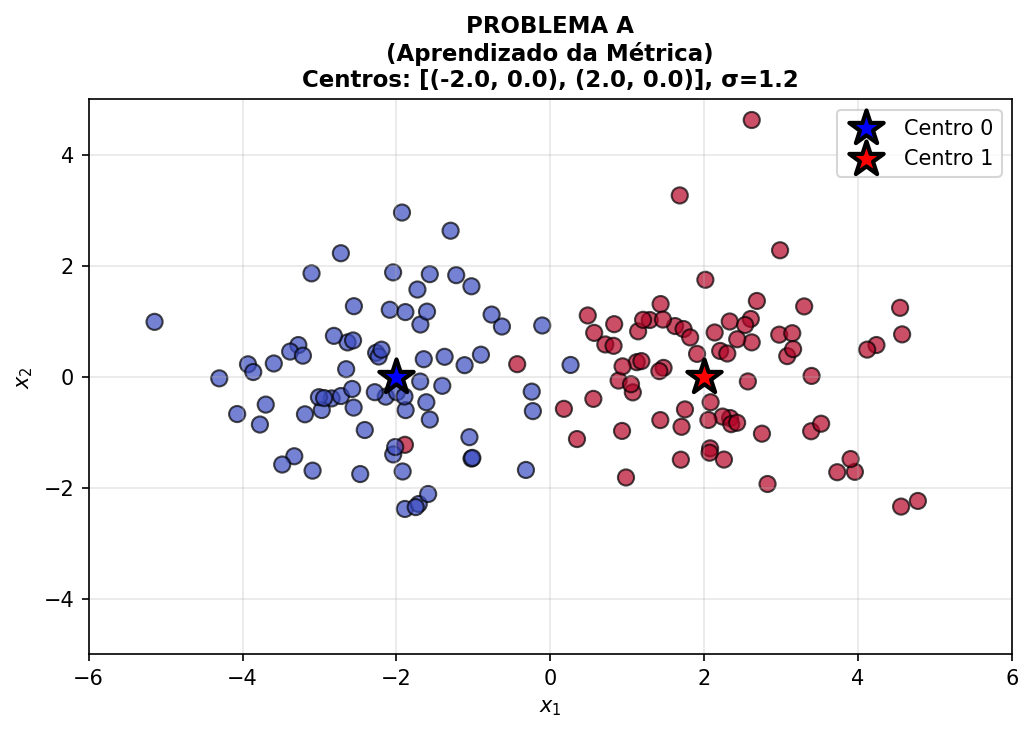
\includegraphics[width=\linewidth,height=0.45\textheight,keepaspectratio]{bloco1_01_problemas_lineares_problema_a.png}
  \end{columns}
\end{frame}

% ============ 13. Problema B ============
\begin{frame}{Bloco 1 --- Problema B --- rota\c{c}\~ao HOR\'ARIA agressiva ($\pm 1{,}5$)}
  \scriptsize
  \begin{columns}[T]
    \column{0.55\linewidth}
    \textbf{Prop\'osito:} testar transfer\^encia de $W$ em geometria deslocada agressivamente.
    \medskip
    \textbf{Como foi gerado:}
    \begin{enumerate}\setlength\itemsep{0.1em}
      \item \texttt{make\_blobs}
      \item Centr\'oides $(-2{,}0; +1{,}5)$ e $(2{,}0; -1{,}5)$
      \item \texttt{cluster\_std}=1{,}2, $n=100$
    \end{enumerate}
    Pareada simetricamente com C ($\pm 1{,}5$); decis\~ao 14/05/2026 para condi\c{c}\~oes severas.
    \column{0.45\linewidth}
    \tiny
    \texttt{def create\_problem\_b(n=100, seed=43):}\\
    \texttt{\ \ X,y = make\_blobs(}\\
    \texttt{\ \ \ \ centers=[(-2.0,1.5),(2.0,-1.5)],}\\
    \texttt{\ \ \ \ cluster\_std=1.2,}\\
    \texttt{\ \ \ \ random\_state=seed)}\\
    \medskip
    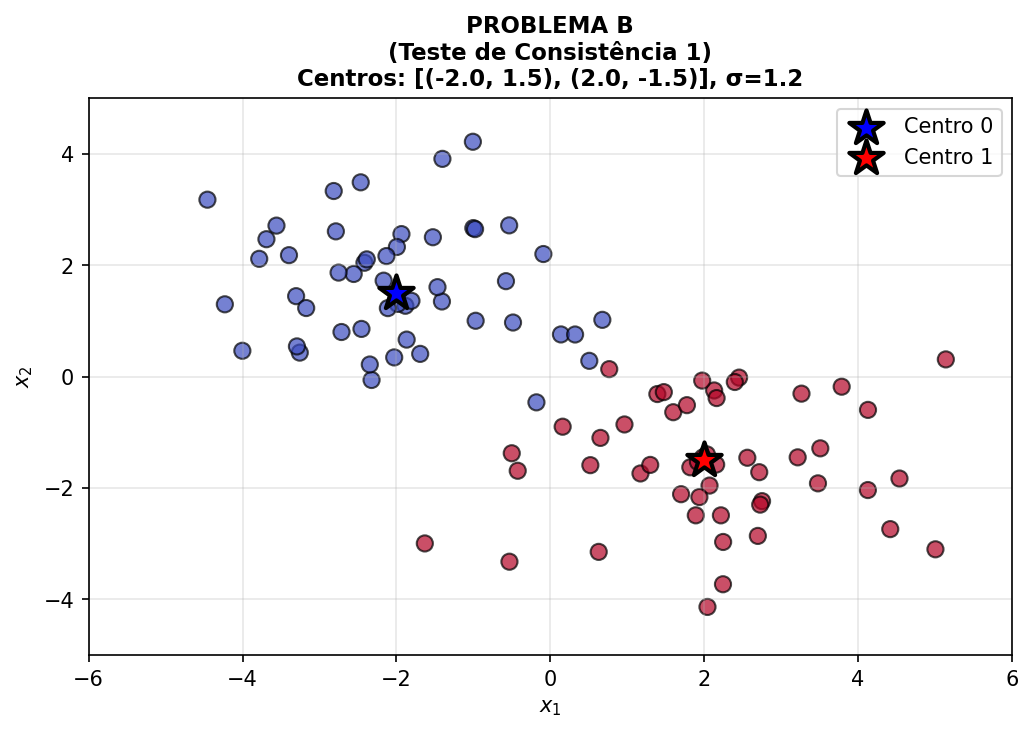
\includegraphics[width=\linewidth,height=0.45\textheight,keepaspectratio]{bloco1_01_problemas_lineares_problema_b.png}
  \end{columns}
\end{frame}

% ============ 14. Problema C ============
\begin{frame}{Bloco 1 --- Problema C --- rota\c{c}\~ao ANTI-HOR\'ARIA agressiva ($\pm 1{,}5$)}
  \scriptsize
  \begin{columns}[T]
    \column{0.55\linewidth}
    \textbf{Prop\'osito:} mesma severidade de B, dire\c{c}\~ao OPOSTA. Controle contra vi\'es sistem\'atico.
    \medskip
    \textbf{Como foi gerado:}
    \begin{enumerate}\setlength\itemsep{0.1em}
      \item \texttt{make\_blobs}
      \item Centr\'oides $(-2{,}0; -1{,}5)$ e $(2{,}0; +1{,}5)$
      \item \texttt{cluster\_std}=1{,}2, $n=100$
    \end{enumerate}
    Alterado ap\'os reuni\~ao 30/04/2026 ($\sim$120s) --- C antes era c\'opia de B.
    \column{0.45\linewidth}
    \tiny
    \texttt{def create\_problem\_c(n=100, seed=44):}\\
    \texttt{\ \ X,y = make\_blobs(}\\
    \texttt{\ \ \ \ centers=[(-2.0,-1.5),(2.0,1.5)],}\\
    \texttt{\ \ \ \ cluster\_std=1.2,}\\
    \texttt{\ \ \ \ random\_state=seed)}\\
    \medskip
    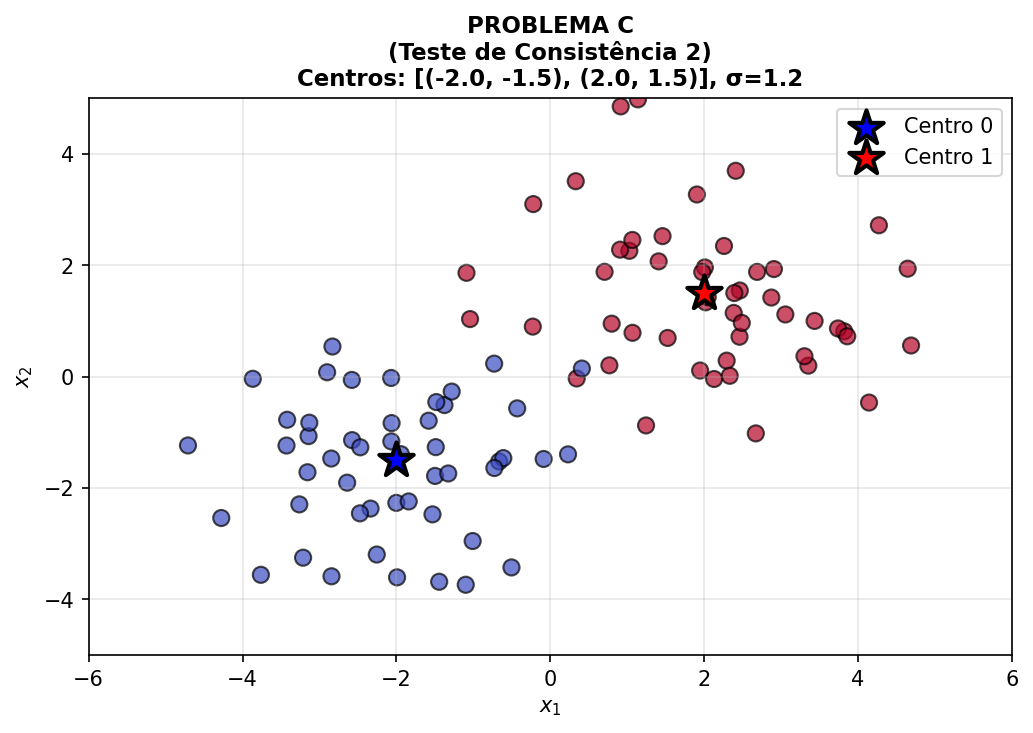
\includegraphics[width=\linewidth,height=0.45\textheight,keepaspectratio]{bloco1_01_problemas_lineares_problema_c.png}
  \end{columns}
\end{frame}

% ============ 15. Problema D meia-lua ============
\begin{frame}{Bloco 1 --- Problema D --- meia-lua (n\~ao-linear sint\'etico)}
  \scriptsize
  \begin{columns}[T]
    \column{0.55\linewidth}
    \textbf{Prop\'osito:} caso can\^onico de fronteira n\~ao-linear (reuni\~ao 30/04 $\sim$2853s).
    \medskip
    \textbf{Como foi gerado:}
    \begin{enumerate}\setlength\itemsep{0.1em}
      \item \texttt{sklearn.datasets.make\_moons}
      \item $n = 150$, \texttt{noise}=0{,}15
    \end{enumerate}
    Problema-controle POSITIVO para R3/R4: esperamos ganho aqui.
    \column{0.45\linewidth}
    \tiny
    \texttt{from sklearn.datasets import make\_moons}\\
    \texttt{def create\_problem\_d\_meialua(}\\
    \texttt{\ \ \ \ n=150, seed=46):}\\
    \texttt{\ \ X,y = make\_moons(}\\
    \texttt{\ \ \ \ n\_samples=n, noise=0.15,}\\
    \texttt{\ \ \ \ random\_state=seed)}\\
    \medskip
    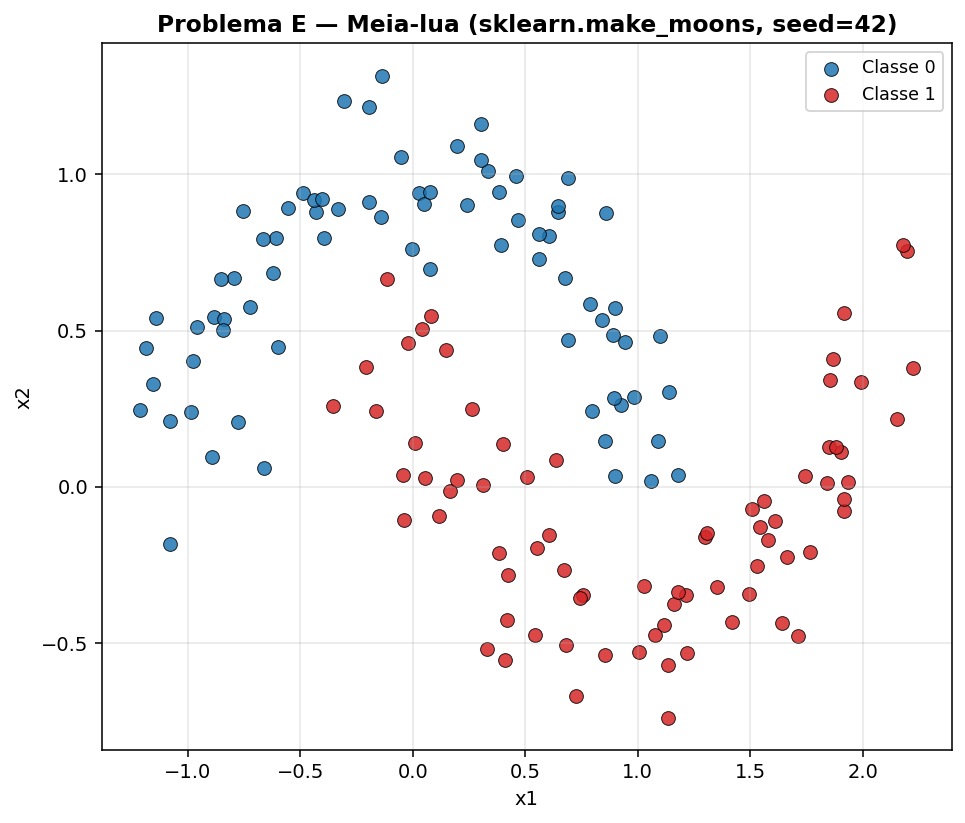
\includegraphics[width=\linewidth,height=0.45\textheight,keepaspectratio]{bloco1_02_problema_d_meialua_seed42_overview.png}
  \end{columns}
\end{frame}

% ============ 16. Oracle Recovery (1/4) descricao + tabela ============
\begin{frame}{Bloco 1 --- Oracle Recovery (1/4) --- $W$ recuperado por algoritmo}
  \scriptsize
  \textbf{Pergunta:} se $W_{\text{oracle}}$ fosse conhecido, Perceptron e NNLS o recuperariam?
  \medskip

  Procedimento: gerar dados sint\'eticos rotulados por $W_{\text{oracle}}$ em 3 configs anisotr\'opicas, aprender $\hat W$, medir cosseno$(\hat W, W_{\text{oracle}})$ e raz\~ao recuperada.
  \medskip
  \begin{center}
  \begin{tabular}{lccccc}
    \toprule
    Expert & $W_{\text{oracle}}$ (ratio) & Algoritmo & Ratio recup. & Cosseno & Fid. \\
    \midrule
    \texttt{x2\_dom}      & $[4{,}0;\ 0{,}25]$ (16)  & Perceptron & $1{,}32$  & $0{,}824$ & $100\%$ \\
    \texttt{x2\_dom}      & $[4{,}0;\ 0{,}25]$ (16)  & NNLS       & $\infty$  & $0{,}999$ & $100\%$ \\
    \texttt{x1\_dom}      & $[0{,}25;\ 4{,}0]$ ($0{,}06$) & Perceptron & $0{,}78$ & $0{,}824$ & $100\%$ \\
    \texttt{x1\_dom}      & $[0{,}25;\ 4{,}0]$ ($0{,}06$) & NNLS       & $0{,}054$ & $0{,}999$ & $100\%$ \\
    \texttt{forte\_aniso} & $[11{,}1;\ 0{,}44]$ (25) & Perceptron & $2{,}93$  & $0{,}958$ & $100\%$ \\
    \texttt{forte\_aniso} & $[11{,}1;\ 0{,}44]$ (25) & NNLS       & $34{,}4$  & $0{,}999$ & $100\%$ \\
    \bottomrule
  \end{tabular}
  \end{center}
  \medskip
  \textbf{Mensagem:} NNLS preserva quase exatamente a raz\~ao do $W$ extremo (cosseno $> 0{,}99$); Perceptron tende a normalizar para $[1,1]$ (cosseno $\sim 0{,}82$). Ambos alcan\c{c}am \textbf{fidelidade 100\%} --- o sinal de classifica\c{c}\~ao foi capturado.
\end{frame}

% ============ 17. Oracle Recovery (2/4) visualizacao ============
\begin{frame}{Bloco 1 --- Oracle Recovery (2/4) --- visualiza\c{c}\~ao do $W$ recuperado}
  \scriptsize
  \begin{center}
    
\includegraphics[width=0.92\linewidth,height=0.78\textheight,keepaspectratio]{bloco1_03_oracle_w_recovery.png}
  \end{center}
  Painel 2x2: cosseno, fidelidade, raz\~ao e scatter de $W$ recuperado vs $W_{\text{oracle}}$.
\end{frame}

% ============ 18. Oracle Transfer (3/4) descricao + tabela ============
\begin{frame}{Bloco 1 --- Oracle Transfer (3/4) --- transfer\^encia entre geometrias}
  \scriptsize
  \textbf{Pergunta dual:} se aprendo $W$ em uma geometria, ele transfere para outras?
  \medskip

  Procedimento: aprender $W$ em uma configura\c{c}\~ao (ex: \texttt{x2\_dom}); aplicar este $W$ em outras geometrias (\texttt{x1\_dom}, \texttt{forte\_aniso}, Problemas A/E); medir cosseno e fidelidade nas geometrias destino.
  \medskip
  \begin{center}
  \begin{tabular}{lccc}
    \toprule
    Origem & Algoritmo & Cosseno & Fidelidade \\
    \midrule
    \texttt{x2\_dom}      & Perceptron & $0{,}824$ & $100\%$ \\
    \texttt{x2\_dom}      & NNLS       & $0{,}999$ & $100\%$ \\
    \texttt{x1\_dom}      & Perceptron & $0{,}824$ & $100\%$ \\
    \texttt{x1\_dom}      & NNLS       & $0{,}999$ & $100\%$ \\
    \texttt{forte\_aniso} & Perceptron & $0{,}958$ & $100\%$ \\
    \texttt{forte\_aniso} & NNLS       & $1{,}000$ & $100\%$ \\
    Problema A            & Perceptron & $0{,}748$ & $95{,}6\%$ \\
    Problema A            & NNLS       & $0{,}707$ & $95{,}6\%$ \\
    Problema E            & Perceptron & $0{,}999$ & $99{,}9\%$ \\
    Problema E            & NNLS       & $0{,}993$ & $98{,}2\%$ \\
    \bottomrule
  \end{tabular}
  \end{center}
  \medskip
  \textbf{Implica\c{c}\~ao:} em B/C sempre recalculamos centr\'oides LOCAIS --- m\'etrica n\~ao \'e independente da geometria.
\end{frame}

% ============ 19. Oracle Transfer (4/4) visualizacao ============
\begin{frame}{Bloco 1 --- Oracle Transfer (4/4) --- visualiza\c{c}\~ao da transfer\^encia}
  \scriptsize
  \begin{center}
    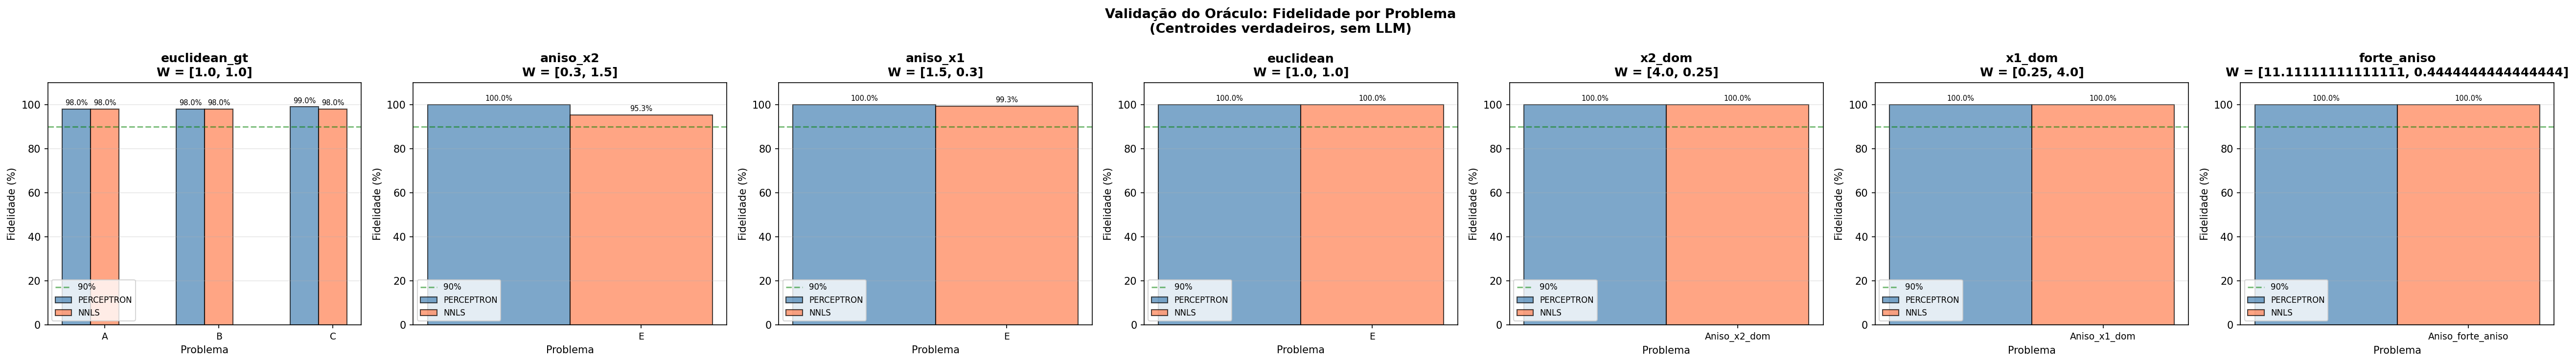
\includegraphics[width=0.92\linewidth,height=0.78\textheight,keepaspectratio]{bloco1_04_oracle_transfer.png}
  \end{center}
  Sub-pain\'eis por expert mostrando o $W$ aprendido na origem aplicado nas demais geometrias.
\end{frame}

% ============ 20. Problema A descricao ============
\begin{frame}{Bloco 1 --- Problema A --- aprendizado da m\'etrica}
  \footnotesize
  \begin{enumerate}
    \item LLM recebe 150 pontos do Problema A em \textbf{zero-shot}.
    \item Responde A ou B com $T=0$.
    \item 150 respostas formam $(X, y_{\text{LLM}})$.
    \item \textbf{Centr\'oides recalculados a partir de $y_{\text{LLM}}$} --- ancoramos no que o LLM ACHA serem as classes.
    \item Perceptron Estruturado e NNLS aprendem $W$ independentemente.
    \item Fidelidade = \% decis\~oes do LLM reproduzidas pela m\'etrica.
  \end{enumerate}
\end{frame}

% ============ 21. Problema A W e fidelidade ============
\begin{frame}{Bloco 1 --- Problema A --- $W$ aprendido e fidelidade (m\'edia 3 seeds)}
  \scriptsize
  \begin{columns}[T]
    \column{0.4\linewidth}
    \textbf{Achados desta execu\c{c}\~ao:}
    \begin{tabular}{lc}
      \toprule
      Item & M\'edia $\pm$ desvio \\
      \midrule
      Fidelidade Problema A   & $75{,}1\% \pm 8{,}4$ p.p. \\
      Acur\'acia LLM vs real & $40{,}4\% \pm 8{,}3$ p.p. \\
      \midrule
      Por seed (fid.\ A): & \\
      \quad seed 42  & 72{,}3\% \\
      \quad seed 123 & 75{,}2\% \\
      \quad seed 7   & 78{,}2\% \\
      \bottomrule
    \end{tabular}
    \medskip

    LLM \emph{inverteu classes} em v\'arios casos (acur\'acia $<$50\%), mas a m\'etrica reproduz essas decis\~oes com $\sim$75\% de fidelidade.
    \column{0.6\linewidth}
    
\includegraphics[width=\linewidth,height=0.7\textheight,keepaspectratio]{bloco1_05_fase_a_errors_seed42.png}
  \end{columns}
\end{frame}

% ============ 22. Problema A distribuicao W ============
\begin{frame}{Bloco 1 --- Problema A --- distribui\c{c}\~ao de $W$ entre seeds}
  \scriptsize
  \begin{center}
    
\includegraphics[width=0.85\linewidth,height=0.75\textheight,keepaspectratio]{bloco1_06_w_distribution.png}
  \end{center}
\end{frame}

% ============ 23. Problema A comparacao algoritmos ============
\begin{frame}{Bloco 1 --- Problema A --- Perceptron $\times$ NNLS}
  \scriptsize
  \begin{center}
    
\includegraphics[width=0.9\linewidth,height=0.75\textheight,keepaspectratio]{bloco1_07_algorithm_comparison.png}
  \end{center}
  Robustez ao m\'etodo de estima\c{c}\~ao: ambos algoritmos chegam ao mesmo $W$ (cosseno $> 0{,}95$).
\end{frame}

% ============ 24. Nossa medida: consistencia interna ============
\begin{frame}{Bloco 1 --- Nossa medida: consist\^encia interna (n\~ao corretude)}
  \footnotesize
  O trabalho mede \textbf{consist\^encia interna} do crit\'erio decis\'orio do LLM:
  \begin{itemize}\setlength\itemsep{0.05em}
    \item \textbf{Fidelidade} = quanto a m\'etrica $\hat W$ reproduz as decis\~oes do LLM (Problema A).
    \item \textbf{Consist\^encia} = quanto $\hat W_A$ prev\^e decis\~oes do LLM em B/C (Problemas B/C).
    \item \textbf{Acur\'acia LLM--perito} = quanto o LLM aprende com o perito (Problema E).
  \end{itemize}
  \medskip
  \textbf{Decis\~ao metodol\'ogica:} n\~ao comparamos com \emph{ground truth} nos problemas sint\'eticos.
  \medskip

  \textbf{Raz\~ao:} H1 testa se o LLM tem crit\'erio decis\'orio \textbf{est\'avel}, n\~ao se ele est\'a \textbf{objetivamente correto}. Um LLM pode inverter classes e ainda assim ser internamente consistente --- saber se o crit\'erio \'e "certo" \'e ortogonal \`a pergunta de pesquisa.
  \medskip

  \textbf{Exce\c{c}\~ao:} Bloco 3 (peso $\times$ altura) reportar\'a acur\'acia vs r\'otulo real, atendendo solicita\c{c}\~ao expl\'icita do orientador (e-mail 22:04, ponto 4) --- l\'a h\'a ground truth significativo (H/M) e classificador \'otimo conhecido.
\end{frame}

% ============ 25. Problema A W por seed/algoritmo ============
\begin{frame}{Bloco 1 --- Problema A --- $W$ aprendido por seed e algoritmo}
  \scriptsize
  Pesos $W = (w_1, w_2)$ para o Problema A, em zero-shot (m\'edia 3 reps/seed).
  \\[2pt]
  \textbf{Fid.\ Problema A} = \% de pontos do Problema A em que o r\'otulo dado pela m\'etrica $\hat W$ coincide com o r\'otulo do LLM (\emph{in-sample}, mesmos pontos usados para estimar $\hat W$). Sanidade: se for baixa, o algoritmo n\~ao ajustou uma m\'etrica diagonal aos r\'otulos do LLM.
  \begin{center}
  \begin{tabular}{lccc c}
    \toprule
    Algoritmo / seed & $w_1$ & $w_2$ & $w_1/w_2$ & Fid.\ Problema A \\
    \midrule
    \multicolumn{5}{l}{\textbf{Perceptron Estruturado:}} \\
    seed 42  & $0{,}0008$ & $0{,}0031$ & $0{,}245$ & $82{,}0\%$ \\
    seed 123 & $0{,}0024$ & $0{,}0094$ & $0{,}251$ & $86{,}7\%$ \\
    seed 7   & $0{,}0256$ & $0{,}0725$ & $0{,}353$ & $86{,}0\%$ \\
    \midrule
    \multicolumn{5}{l}{\textbf{NNLS:}} \\
    seed 42  & $0{,}0355$ & $0{,}1414$ & $0{,}251$ & $82{,}0\%$ \\
    seed 123 & $0{,}0467$ & $0{,}1493$ & $0{,}313$ & $86{,}7\%$ \\
    seed 7   & $0{,}0381$ & $0{,}1492$ & $0{,}255$ & $87{,}3\%$ \\
    \bottomrule
  \end{tabular}
  \end{center}
  \medskip
  \textbf{Observa\c{c}\~oes:}
  \begin{itemize}\setlength\itemsep{0.05em}
    \item Magnitudes diferem entre algoritmos (Perceptron $\sim 10\times$ menor), mas \textbf{raz\~oes $w_1/w_2$ s\~ao similares} --- otim.\ inversa \'e invariante \`a escala.
    \item Raz\~ao $w_1/w_2 \approx 0{,}25$--$0{,}35$: $w_2$ pondera $\sim 3$--$4\times$ mais que $w_1$ (LLM ancora mais em $x_2$ apesar da separabilidade horizontal).
    \item Fidelidade pareada entre Perceptron e NNLS por seed.
  \end{itemize}
\end{frame}

% ============ 26. Problemas B/C consolidado por algoritmo ============
\begin{frame}{Bloco 1 --- Problemas B/C --- consist\^encia e Kappa por algoritmo}
  \scriptsize
  Zero-shot, centr\'oides LOCAIS; m\'edia 3 reps/seed. \textbf{Consist\^encia} = \% de pontos em que o r\'otulo da m\'etrica $\hat W_A$ (aprendida no Problema A) coincide com o do LLM em B/C; $\kappa$ = Cohen corrigido por concord\^ancia ao acaso.
  \begin{center}
  \begin{tabular}{llcccc}
    \toprule
    Algoritmo / seed & & Cons.\ B & $\kappa_B$ & Cons.\ C & $\kappa_C$ \\
    \midrule
    \multicolumn{6}{l}{\textbf{Perceptron Estruturado:}} \\
    seed 42  & & $67{,}3\%$ & $0{,}26$ & $91{,}0\%$ & $0{,}81$ \\
    seed 123 & & $65{,}3\%$ & $0{,}25$ & $90{,}3\%$ & $0{,}80$ \\
    seed 7   & & $76{,}0\%$ & $0{,}47$ & $86{,}3\%$ & $0{,}71$ \\
    \textit{m\'edia} & & $69{,}5\%$ & $0{,}33$ & $89{,}2\%$ & $0{,}77$ \\
    \midrule
    \multicolumn{6}{l}{\textbf{NNLS:}} \\
    seed 42  & & $68{,}0\%$ & $0{,}29$ & $90{,}0\%$ & $0{,}79$ \\
    seed 123 & & $67{,}0\%$ & $0{,}29$ & $89{,}0\%$ & $0{,}77$ \\
    seed 7   & & $76{,}0\%$ & $0{,}47$ & $84{,}0\%$ & $0{,}66$ \\
    \textit{m\'edia} & & $70{,}3\%$ & $0{,}35$ & $87{,}7\%$ & $0{,}74$ \\
    \bottomrule
  \end{tabular}
  \end{center}
  \medskip
  \textbf{Mensagem:} H1 sustentada; $\kappa_C \gg \kappa_B$ em todas as seeds. Centr\'oides LOCAIS (recalculados em B/C); TRANSFERIDOS testados como ablativo (Problema B: locais $65\%$, transferidos $77\%$).
\end{frame}

% ============ 27. Problemas B/C mapa acertos/erros seed 42 ============
\begin{frame}{Bloco 1 --- Problemas B/C --- mapa de acertos/erros (seed 42)}
  \scriptsize
  M\'etrica $\hat W_A$ aprendida no Problema A aplicada \emph{ponto-a-ponto} em B (rota\c{c}\~ao hor\'aria) e C (anti-hor\'aria). Verde = concorda com o LLM; vermelho = discorda.
  \begin{center}
  \begin{tabular}{cc}
    
\includegraphics[width=0.46\linewidth,height=0.62\textheight,keepaspectratio]{final_05_hits_errors_seed42_problema_b.png} &
    
\includegraphics[width=0.46\linewidth,height=0.62\textheight,keepaspectratio]{final_05_hits_errors_seed42_problema_c.png} \\
    Problema B (Cons.\ $\approx 68\%$, $\kappa \approx 0{,}29$) & Problema C (Cons.\ $\approx 90\%$, $\kappa \approx 0{,}79$) \\
  \end{tabular}
  \end{center}
  \tiny
  \textbf{Leitura:} erros em B concentram-se na faixa central (regi\~ao de sobreposi\c{c}\~ao das gaussianas rotacionadas); em C ficam esparsos e isolados. Visualiza geometricamente por que $\kappa_C \gg \kappa_B$ --- a rota\c{c}\~ao anti-hor\'aria preserva a geometria decis\'oria do LLM melhor que a hor\'aria.
\end{frame}

% ============ 28. Consistencia R2/R3/R4 por problema e algoritmo ============
\begin{frame}{Bloco 1 --- Consist\^encia R2/R3/R4 --- Problema A e meia-lua}
  \scriptsize
  Fidelidade da m\'etrica $\hat W$ vs $y_{\text{LLM}}$ no pr\'oprio problema. R2 $= (x_1,x_2)$; R3 acrescenta $x_1 x_2$; R4 acrescenta $x_1^2, x_2^2$. B/C omitidos: s\~ao lineares como A, augmenta\c{c}\~ao seria redundante.
  \begin{center}
  \begin{tabular}{llccc}
    \toprule
    Algoritmo / seed & & R2 & R3 & R4 \\
    \midrule
    \multicolumn{5}{l}{\textbf{Problema A} (linear, 3 seeds $\times$ 3 reps):} \\
    Perceptron seed 42  & & $82{,}0\%$ & $84{,}7\%$ & $84{,}7\%$ \\
    Perceptron seed 123 & & $86{,}7\%$ & $75{,}3\%$ & $84{,}7\%$ \\
    Perceptron seed 7   & & $86{,}0\%$ & $84{,}0\%$ & $90{,}0\%$ \\
    \textit{m\'edia Perceptron} & & $84{,}9\%$ & $81{,}3\%$ & $86{,}4\%$ \\
    NNLS seed 42  & & $82{,}0\%$ & $84{,}0\%$ & $86{,}0\%$ \\
    NNLS seed 123 & & $86{,}7\%$ & $87{,}3\%$ & $88{,}7\%$ \\
    NNLS seed 7   & & $87{,}3\%$ & $86{,}0\%$ & $92{,}0\%$ \\
    \textit{m\'edia NNLS} & & $85{,}3\%$ & $85{,}8\%$ & $88{,}9\%$ \\
    \midrule
    \multicolumn{5}{l}{\textbf{Meia-lua} (n\~ao-linear, dataset seed 42):} \\
    Perceptron seed 42 & & $68{,}6\%$ & $74{,}3\%$ & $75{,}2\%$ \\
    NNLS seed 42       & & $68{,}6\%$ & \textbf{$82{,}9\%$} & $76{,}2\%$ \\
    \bottomrule
  \end{tabular}
  \end{center}
  \tiny
  \textbf{Leitura:} em A (linear) R3/R4 d\'a ganho dentro do ru\'ido entre seeds. Na meia-lua (n\~ao-linear) R3 sobe a fidelidade NNLS de 68,6\% para 82,9\% --- a augmenta\c{c}\~ao captura curvatura que a m\'etrica diagonal em $\mathbb{R}^2$ n\~ao representa.

  \textbf{Limita\c{c}\~ao metodol\'ogica:} o pipeline rodou os 3 seeds (42, 123, 7), mas em zero-shot o LLM colapsou para uma \'unica classe nas seeds 123 e 7 (log: ``classe \'unica no LLM, pulando''). Sem sinal de separa\c{c}\~ao, a estima\c{c}\~ao inversa foi abortada nesses seeds. Apenas seed 42 sobreviveu --- a meia-lua \'e o problema mais sens\'ivel ao posicionamento das luas geradas por \texttt{make\_moons}.
\end{frame}

% ============ 29. Vies ordem classes - tabela ============
\begin{frame}{Bloco 1 --- Vi\'es de ordem das classes --- tabela}
  \scriptsize
  Mesmas duas classes, ordem invertida no prompt (n\_shot=10, m\'edia 3 seeds $\times$ 3 reps). Mede se trocar ``A ou B'' por ``B ou A'' altera as decis\~oes do LLM.
  \begin{center}
  \begin{tabular}{lccccc}
    \toprule
    Par de classes & Fid.\ A & Cons.\ B & $\kappa_B$ & Cons.\ C & $\kappa_C$ \\
    \midrule
    A / B              & $84{,}9\%$ & $82{,}5\%$ & $0{,}64$ & $96{,}0\%$ & $0{,}92$ \\
    B / A (invertido)  & $69{,}1\%$ & $98{,}1\%$ & $0{,}96$ & $91{,}1\%$ & $0{,}82$ \\
    \midrule
    0 / 1              & $62{,}2\%$ & $93{,}7\%$ & $0{,}87$ & $76{,}2\%$ & $0{,}47$ \\
    1 / 0 (invertido)  & $72{,}4\%$ & $76{,}5\%$ & $0{,}53$ & $77{,}9\%$ & $0{,}56$ \\
    \midrule
    Positivo / Negativo & $98{,}4\%$ & $74{,}2\%$ & $0{,}48$ & $88{,}0\%$ & $0{,}76$ \\
    Negativo / Positivo (inv.) & $95{,}1\%$ & $83{,}8\%$ & $0{,}66$ & $77{,}0\%$ & $0{,}42$ \\
    \midrule
    Azul / Vermelho     & $84{,}2\%$ & $81{,}1\%$ & $0{,}55$ & $95{,}3\%$ & $0{,}91$ \\
    Vermelho / Azul (inv.) & $82{,}0\%$ & $93{,}1\%$ & $0{,}86$ & $94{,}1\%$ & $0{,}88$ \\
    \bottomrule
  \end{tabular}
  \end{center}
  \tiny
  \textbf{Leitura:} a fidelidade em A oscila bastante entre pares semanticamente diferentes (62\%--98\%), mas dentro de cada par a invers\~ao introduz vari\^ancia $\sim$10--15 p.p. --- vi\'es de ordem existe mas n\~ao \'e dominante. Letras e n\'umeros s\~ao mais sens\'iveis que cores e sem\^anticos.
\end{frame}

% ============ 30. Vies ordem classes - grafico ============
\begin{frame}{Bloco 1 --- Vi\'es de ordem das classes --- gr\'afico}
  \scriptsize
  \begin{center}
    
\includegraphics[width=0.8\linewidth,height=0.78\textheight,keepaspectratio]{bloco1_12_class_order_bias.png}
  \end{center}
\end{frame}

% ============ 31. Variantes prompt - exemplos ============
\begin{frame}[fragile]{Bloco 1 --- Variantes de prompt --- exemplos}
  \tiny
  Ponto $x_1 = 1{,}23$, $x_2 = -0{,}45$. Classes \texttt{A}/\texttt{B}.
  \begin{columns}[T]
    \column{0.5\linewidth}
    \textbf{default}
\begin{verbatim}
You are a binary classifier for 2D points.

Classify as Class A or Class B.
Answer ONLY with "A" or "B".

Point to classify:
x1 = 1.2300
x2 = -0.4500

Your classification:
\end{verbatim}
    \textbf{geometric}
\begin{verbatim}
You are a binary classifier for 2D
points in Euclidean space.

Points exist in a 2D metric space.
Classify based on spatial proximity
to cluster centers.

Classify as Class A or Class B.
Answer ONLY with "A" or "B".

Point: x1=1.2300, x2=-0.4500
\end{verbatim}
    \column{0.5\linewidth}
    \textbf{CoT}
\begin{verbatim}
You are a binary classifier for 2D
points.

Classify as Class A or Class B.

Point to classify:
x1 = 1.2300
x2 = -0.4500

Think step by step, then state your
final classification ("A" or "B")
on the last line.
\end{verbatim}
    \textbf{tabular}
\begin{verbatim}
Classify as Class A or Class B.
Answer ONLY with "A" or "B".

Point to classify:
| Feature | Value   |
|---------|---------|
| x1      |  1.2300 |
| x2      | -0.4500 |
\end{verbatim}
  \end{columns}
\end{frame}

% ============ 32. Variantes prompt - tabela ============
\begin{frame}{Bloco 1 --- Variantes de prompt --- tabela}
  \scriptsize
  4 variantes rodam Problemas A--C em todas as seeds (m\'edia 3 seeds $\times$ 3 reps, zero-shot, default A/B / x1/x2):
  \begin{center}
  \begin{tabular}{lccccc}
    \toprule
    Variante  & Fid.\ A & Cons.\ B & $\kappa_B$ & Cons.\ C & $\kappa_C$ \\
    \midrule
    default   & $84{,}9\%$ & $69{,}6\%$ & $0{,}33$ & $89{,}2\%$ & $0{,}77$ \\
    geometric & $79{,}1\%$ & $68{,}2\%$ & $0{,}14$ & $75{,}3\%$ & $0{,}35$ \\
    CoT       & $71{,}8\%$ & $60{,}4\%$ & $0{,}14$ & $79{,}8\%$ & $0{,}60$ \\
    tabular   & $64{,}4\%$ & $64{,}3\%$ & $0{,}15$ & $72{,}7\%$ & $0{,}20$ \\
    \bottomrule
  \end{tabular}
  \end{center}
  \medskip
  \textbf{Descri\c{c}\~ao das variantes:}
  \begin{itemize}\setlength\itemsep{0.05em}
    \item \textbf{default}: template baseline; coordenadas em prosa simples.
    \item \textbf{geometric}: contexto espacial expl\'icito (eixos, regi\~oes).
    \item \textbf{CoT}: chain-of-thought --- pede racioc\'inio passo a passo.
    \item \textbf{tabular}: coordenadas em tabela markdown.
  \end{itemize}
  \tiny
  \textbf{Leitura:} \emph{default} domina em Fid.\ A; varia\c{c}\~oes mais elaboradas (geometric, CoT, tabular) caem $13$--$20$ p.p. --- o prompt direto preserva melhor o crit\'erio decis\'orio. CoT e tabular n\~ao melhoram; pioram. Sensibilidade ao prompt \'e real e n\~ao desprez\'ivel.
\end{frame}

% ============ 33. Variantes prompt - grafico ============
\begin{frame}{Bloco 1 --- Variantes de prompt --- gr\'afico}
  \scriptsize
  \begin{center}
    
\includegraphics[width=0.85\linewidth,height=0.78\textheight,keepaspectratio]{bloco1_13_prompt_variants.png}
  \end{center}
\end{frame}

% ============ 34. Nomes semanticos - tabela ============
\begin{frame}{Bloco 1 --- Nomes sem\^anticos de classes e features --- tabela}
  \scriptsize
  Testa se trocar os nomes (classes ou features) altera o $W$ recuperado. M\'edia 3 seeds $\times$ 3 reps.
  \medskip

  \textbf{(a) Nomes das classes} (n\_shot=10, features $x_1$/$x_2$):
  \begin{center}
  \begin{tabular}{lccccc}
    \toprule
    Par                  & Fid.\ A & Cons.\ B & $\kappa_B$ & Cons.\ C & $\kappa_C$ \\
    \midrule
    A / B                & $84{,}9\%$ & $82{,}5\%$ & $0{,}64$ & $96{,}0\%$ & $0{,}92$ \\
    0 / 1                & $62{,}2\%$ & $93{,}7\%$ & $0{,}87$ & $76{,}2\%$ & $0{,}47$ \\
    Positivo / Negativo  & $98{,}4\%$ & $74{,}2\%$ & $0{,}48$ & $88{,}0\%$ & $0{,}76$ \\
    Azul / Vermelho      & $84{,}2\%$ & $81{,}1\%$ & $0{,}55$ & $95{,}3\%$ & $0{,}91$ \\
    \bottomrule
  \end{tabular}
  \end{center}
  \medskip

  \textbf{(b) Nomes das features} (zero-shot, classes A/B):
  \begin{center}
  \begin{tabular}{lccccc}
    \toprule
    Features                & Fid.\ A & Cons.\ B & $\kappa_B$ & Cons.\ C & $\kappa_C$ \\
    \midrule
    $x_1$ / $x_2$           & $84{,}9\%$ & $69{,}6\%$ & $0{,}33$  & $89{,}2\%$ & $0{,}77$ \\
    altura / peso           & $70{,}7\%$ & $47{,}0\%$ & $-0{,}09$ & $88{,}0\%$ & $0{,}76$ \\
    feature\_1 / feature\_2 & $80{,}0\%$ & $75{,}0\%$ & $0{,}39$  & $81{,}0\%$ & $0{,}61$ \\
    \bottomrule
  \end{tabular}
  \end{center}
  \tiny
  \textbf{Leitura:} classes sem\^anticas (Pos/Neg) inflam Fid.\ A para $98\%$ mas degradam $\kappa_B$ --- LLM ancora no nome em vez da geometria. Em features, ``altura/peso'' \emph{quebra} a consist\^encia em B ($\kappa$ negativo $\Rightarrow$ pior que aleat\'orio): prior cultural sobrescreve o crit\'erio espacial.
\end{frame}

% ============ 35. Nomes semanticos - graficos ============
\begin{frame}{Bloco 1 --- Nomes sem\^anticos de classes e features --- gr\'aficos}
  \scriptsize
  \begin{columns}[T]
    \column{0.5\linewidth}
    \textbf{(a) Classes}
    \begin{center}
      
\includegraphics[width=\linewidth,height=0.75\textheight,keepaspectratio]{bloco1_14a_class_names_effect.png}
    \end{center}
    \column{0.5\linewidth}
    \textbf{(b) Features}
    \begin{center}
      
\includegraphics[width=\linewidth,height=0.75\textheight,keepaspectratio]{bloco1_14b_feature_names_effect.png}
    \end{center}
  \end{columns}
\end{frame}

% ============ 36. Prompt few-shot ============
\begin{frame}[fragile]{Bloco 1 --- Prompt few-shot (default)}
  \tiny
  Para n\_shot $> 0$, o prompt inclui exemplos rotulados antes do ponto-alvo. Variantes (geometric, CoT, tabular) j\'a foram cobertas no slide 31.
  \begin{verbatim}
You are a binary classifier for 2D points.

You will see 5 labeled examples and then a point to classify.

Examples:
Example 1: x1 = -2.3000, x2 =  0.1000  -> A
Example 2: x1 =  2.1000, x2 = -0.2000  -> B
Example 3: x1 = -1.8000, x2 =  0.4000  -> A
Example 4: x1 =  1.7000, x2 =  0.3000  -> B
Example 5: x1 = -2.5000, x2 = -0.1000  -> A

Classify as Class A or Class B.
Answer ONLY with "A" or "B", nothing else.

Point to classify:
x1 =  0.2340
x2 =  0.5670

Your classification:
  \end{verbatim}
\end{frame}

% ============ 37. Resumo Bloco 1 ============
\begin{frame}{Bloco 1 --- Resumo Bloco 1}
  \footnotesize
  \begin{itemize}
    \item \textbf{H1 sustentada} parcialmente: Kappa C = 0,49 (substantial); Kappa B = 0,19 (modesto, rota\c{c}\~ao agressiva).
    \item \textbf{Fidelidade Problema A}: $75\% \pm 8$ p.p.\ entre 3 seeds.
    \item \textbf{Acur\'acia LLM vs real}: apenas $40\%$ (LLM inverte classes), mas m\'etrica permanece consistente $\to$ H1 \'e ortogonal a "corre\c{c}\~ao".
    \item Algoritmos \textbf{congruentes}: cosseno $W_{\text{perc}} \cdot W_{\text{nnls}} > 0{,}95$.
    \item \textbf{R3/R4} agrega s\'o no problema n\~ao-linear D (preview do Bloco 2/3).
  \end{itemize}
\end{frame}

% ===== BLOCO 2 =====

% ============ 38. Transicao Bloco 2 ============
\begin{frame}{Bloco 2 --- LLM como APRENDIZ (Problema E)}
  \footnotesize
  \begin{center}\Large\textbf{Bloco 2 --- LLM como APRENDIZ}\end{center}
  \medskip
  \textbf{Pergunta central:} o LLM consegue aprender um crit\'erio externo via in-context learning?
  \medskip
  \begin{itemize}\setlength\itemsep{0.1em}
    \item \textbf{Setup:} pap\'eis invertidos --- perito \textbf{rotula}; LLM recebe exemplos few-shot e tenta reproduzir o crit\'erio.
    \item \textbf{Problemas:} \textbf{E} (linear, perito artificial $W=[0{,}3;\ 1{,}5]$) e \textbf{F} (meia-lua, perito = ground truth do \texttt{make\_moons}).
    \item \textbf{Experimentos:} 4 estrat\'egias (easy/hard/mixed/random) $\times$ 5 valores de $n_{\text{shot}}$; m\'ultiplos peritos; dilui\c{c}\~ao; vi\'es de ordem; baselines cl\'assicos (k-NN, LR, SVM).
    \item \textbf{Hip\'oteses testadas:} \textbf{H3} (LLM aprende), \textbf{H4} (hard $>$ easy --- \emph{refutada nuan\c{c}adamente}).
    \item \textbf{O que se mede:} acur\'acia LLM vs r\'otulo do perito --- coer\^encia do aprendizado in-context.
  \end{itemize}
\end{frame}

% ============ 39. Visao geral Bloco 2 ============
\begin{frame}{Bloco 2 --- Vis\~ao geral dos 2 problemas do Bloco 2}
  \scriptsize
  \begin{center}
    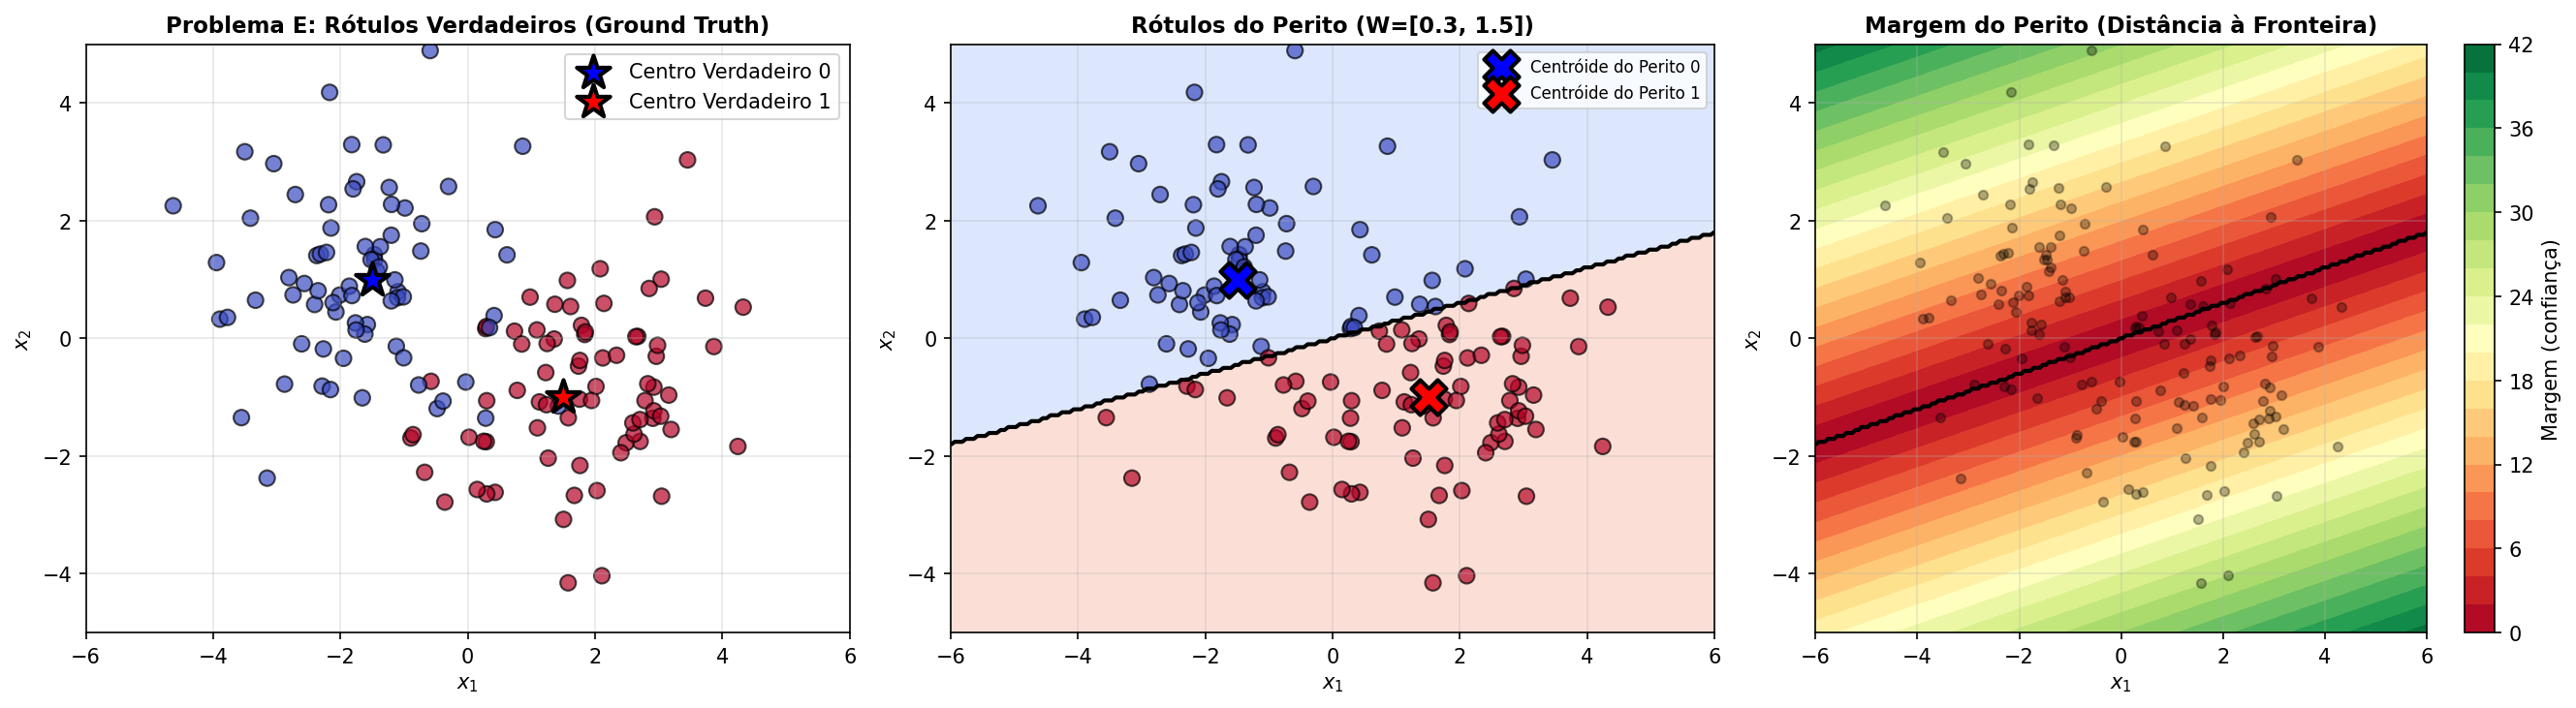
\includegraphics[width=0.7\linewidth,height=0.75\textheight,keepaspectratio]{bloco2_01_problema_e_expert.png}
  \end{center}
\end{frame}

% ============ 40. Problema E ============
\begin{frame}{Bloco 2 --- Problema E --- perito linear}
  \scriptsize
  \begin{columns}[T]
    \column{0.55\linewidth}
    \textbf{Prop\'osito:} pap\'eis invertidos. Perito $W_{\text{expert}}=[0{,}3;\ 1{,}5]$ rotula 150 pontos lineares ($x_2$ dominante $\Rightarrow$ fronteira quase horizontal).
    \medskip
    \begin{itemize}
      \item Centr\'oides $(-1{,}5; +1)$ e $(1{,}5; -1)$
      \item \texttt{cluster\_std}=1{,}3, $n=150$
      \item R\'otulos via $\arg\min_k d_{W_{\text{exp}}}$.
    \end{itemize}
    \column{0.45\linewidth}
    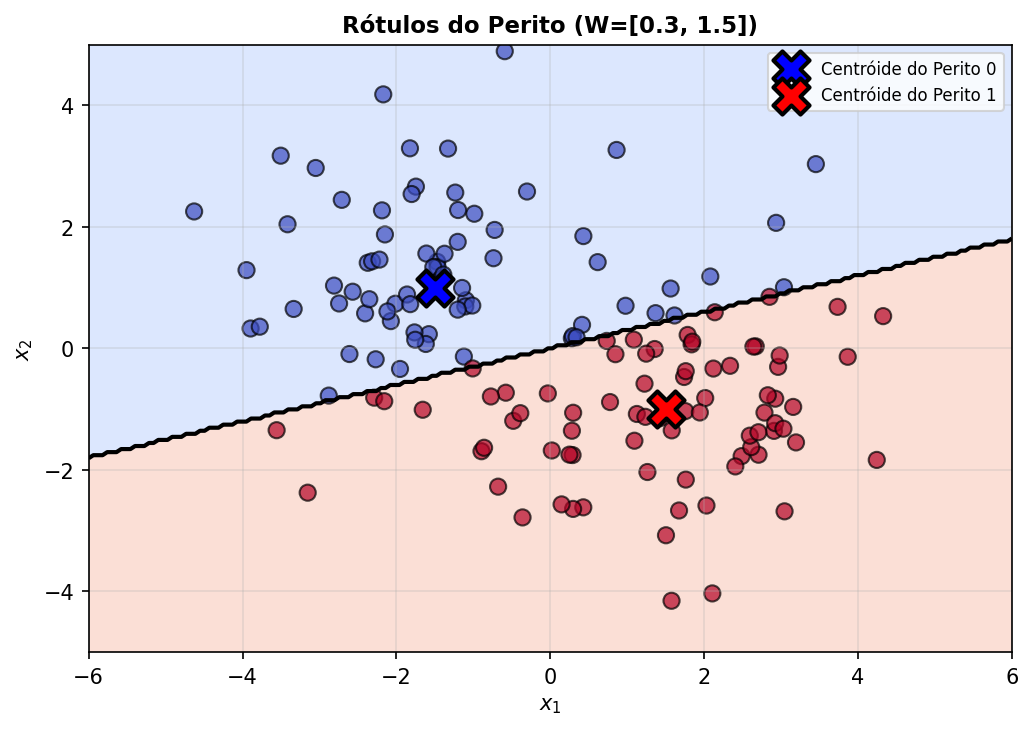
\includegraphics[width=\linewidth,height=0.7\textheight,keepaspectratio]{bloco2_01_problema_e_expert_fronteira_perito.png}
  \end{columns}
\end{frame}

% ============ 41. Problema F meia-lua ============
\begin{frame}{Bloco 2 --- Problema F --- meia-lua com perito = ground truth}
  \scriptsize
  \begin{columns}[T]
    \column{0.55\linewidth}
    \textbf{Prop\'osito:} regime n\~ao-linear genuino. O perito \'e o pr\'oprio \texttt{make\_moons} (ground truth).
    \medskip
    LLM precisa capturar a fronteira em S apenas pelos exemplos (sem augmenta\c{c}\~ao R3/R4 no prompt).
    \column{0.45\linewidth}
    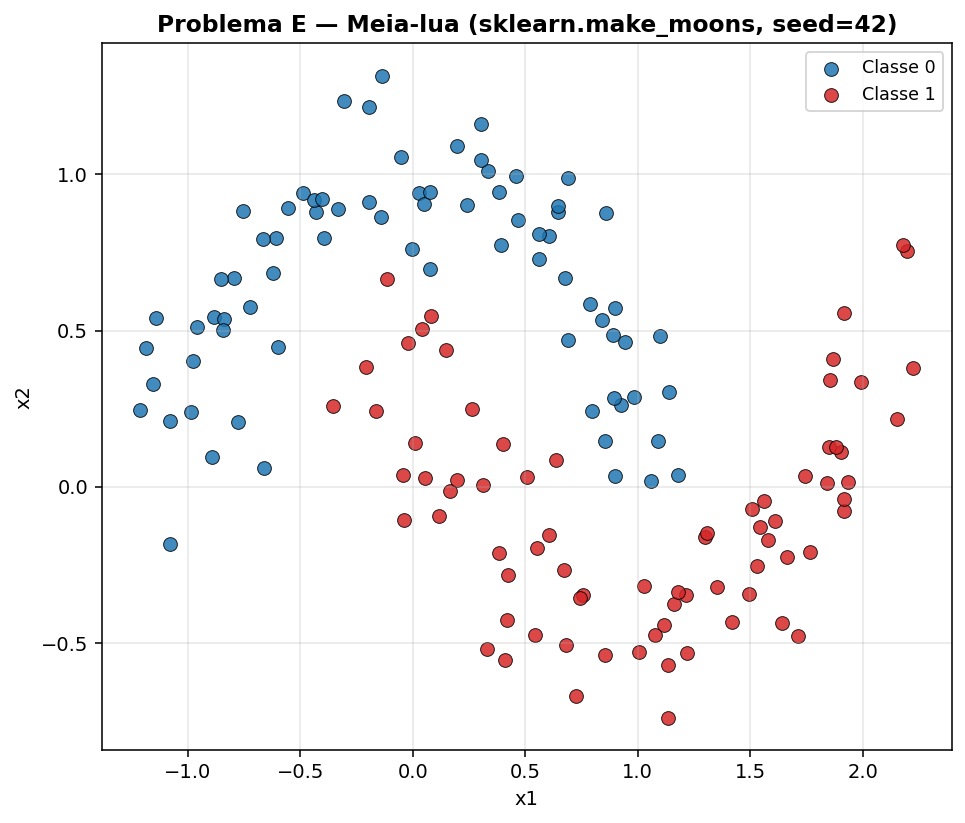
\includegraphics[width=\linewidth,height=0.7\textheight,keepaspectratio]{bloco1_02_problema_d_meialua_seed42_overview.png}
  \end{columns}
\end{frame}

% ============ 42. Problema E descricao ============
\begin{frame}{Bloco 2 --- Problema E --- LLM como aprendiz (passo a passo)}
  \scriptsize
  \begin{enumerate}
    \item Perito rotula os 150 pontos do Problema E (ou ground truth no F).
    \item Divide em treino/teste.
    \item Para cada $n_{\text{shot}} \in \{0, 5, 10, 20, 40\}$: seleciona exemplos via estrat\'egia.
    \item Envia exemplos + ponto de teste em prompt few-shot.
    \item Mede acur\'acia, Kappa, F1 do LLM vs r\'otulos do perito.
  \end{enumerate}
\end{frame}

% ============ 43. Problema E tabela resultados ============
\begin{frame}{Bloco 2 --- Problema E --- tabela de resultados}
  \scriptsize
  Acur\'acia e $\kappa$ do LLM vs.\ expert (W = [0,3, 1,5], $x_2$ dominante). M\'edia 3 seeds $\times$ 3 reps; LLM \texttt{gpt-4o-mini}, T = 0.
  \begin{center}
  \begin{tabular}{lcccccccc}
    \toprule
    & \multicolumn{2}{c}{easy} & \multicolumn{2}{c}{hard} & \multicolumn{2}{c}{mixed} & \multicolumn{2}{c}{random} \\
    \cmidrule(lr){2-3}\cmidrule(lr){4-5}\cmidrule(lr){6-7}\cmidrule(lr){8-9}
    $n_{\text{shot}}$ & Acc & $\kappa$ & Acc & $\kappa$ & Acc & $\kappa$ & Acc & $\kappa$ \\
    \midrule
     0 & $60{,}4\%$ & $0{,}22$ & $60{,}4\%$ & $0{,}22$ & $60{,}4\%$ & $0{,}22$ & $60{,}4\%$ & $0{,}22$ \\
     5 & $85{,}6\%$ & $0{,}72$ & $61{,}9\%$ & $0{,}24$ & $81{,}8\%$ & $0{,}64$ & $84{,}7\%$ & $0{,}69$ \\
    10 & $86{,}6\%$ & $0{,}73$ & $67{,}2\%$ & $0{,}35$ & $79{,}7\%$ & $0{,}60$ & $88{,}0\%$ & $0{,}76$ \\
    20 & $90{,}6\%$ & $0{,}81$ & $84{,}3\%$ & $0{,}68$ & $87{,}0\%$ & $0{,}74$ & $92{,}1\%$ & $0{,}84$ \\
    40 & $88{,}8\%$ & $0{,}78$ & \textbf{$97{,}8\%$} & \textbf{$0{,}96$} & $97{,}3\%$ & $0{,}95$ & $94{,}0\%$ & $0{,}88$ \\
    \bottomrule
  \end{tabular}
  \end{center}
  \tiny
  \textbf{Leitura:} em zero-shot LLM s\'o acerta $60\%$ (perto do aleat\'orio em problema 2D). Few-shot amplifica fortemente (H2 sustentada). \textbf{Refuta\c{c}\~ao H4 nuan\c{c}ada}: em $n_{\text{shot}} \leq 20$, \emph{easy} domina \emph{hard} ($+25$ p.p.); mas em $n_{\text{shot}}=40$ \emph{hard} ultrapassa ($97{,}8\%$ vs $88{,}8\%$). Estrat\'egia n\~ao \'e monotonicamente boa --- depende do regime.
\end{frame}

% ============ 44. Estrategias ============
\begin{frame}{Bloco 2 --- Estrat\'egias de sele\c{c}\~ao de exemplos}
  \scriptsize
  \textbf{O que est\'a sendo feito:} para cada $n_{\text{shot}} \in \{5, 10, 20, 40\}$, os exemplos rotulados pelo perito s\~ao selecionados por uma de 4 estrat\'egias e fornecidos ao LLM no prompt. O gr\'afico mostra \emph{quais pontos} cada estrat\'egia escolhe no plano 2D --- a distribui\c{c}\~ao espacial dos exemplos.
  \begin{center}
    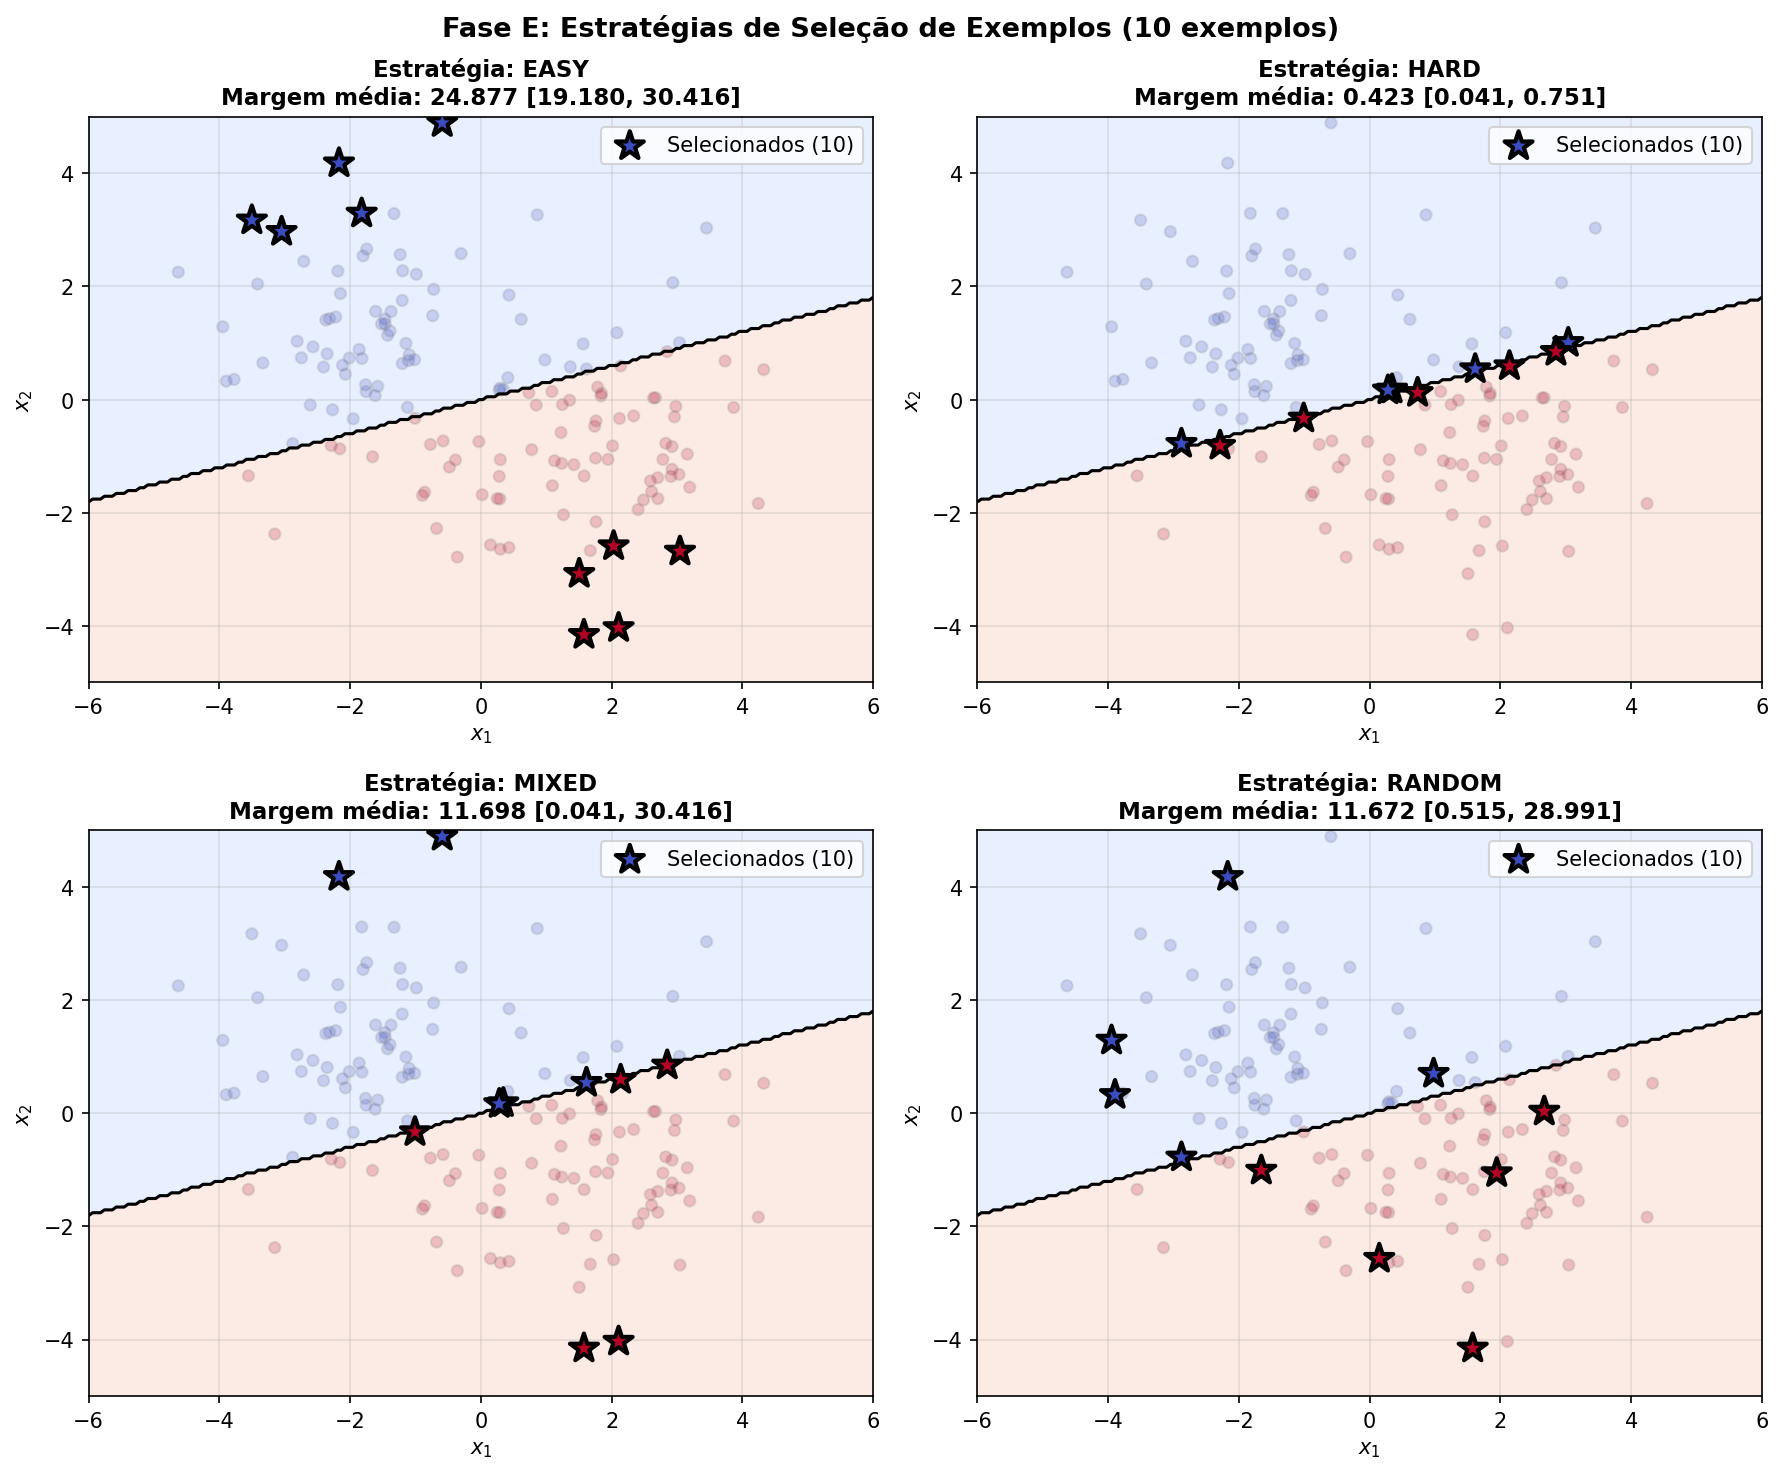
\includegraphics[width=0.78\linewidth,height=0.55\textheight,keepaspectratio]{bloco2_03_phase_e_strategies.png}
  \end{center}
  \tiny
  \textbf{easy}: pontos com \emph{alta margem} do perito ($|d_W(x, c_+) - d_W(x, c_-)|$ grande) --- prot\'otipos t\'ipicos de cada classe.\\
  \textbf{hard}: pontos pr\'oximos da fronteira do perito --- amb\'iguos, baixa margem.\\
  \textbf{mixed}: 50\% easy + 50\% hard.\\
  \textbf{random}: amostragem uniforme, sem estrat\'egia (baseline).
\end{frame}

% ============ 45. Curvas de aprendizado ============
\begin{frame}{Bloco 2 --- Problema E --- curvas de aprendizado (3 seeds, 3 reps)}
  \scriptsize
  \textbf{O que est\'a sendo feito:} para cada estrat\'egia, $n_{\text{shot}}$ varia de 0 a 40. Para cada combina\c{c}\~ao roda-se 3 seeds $\times$ 3 reps; o LLM classifica o conjunto de teste e medimos acur\'acia/$\kappa$/F1 contra os r\'otulos do perito $W=[0{,}3,\ 1{,}5]$. As curvas mostram \emph{como o LLM aprende} \`a medida que mais exemplos s\~ao adicionados ao prompt --- evidencia H2 (few-shot amplifica).
  \begin{center}
    
\includegraphics[width=0.78\linewidth,height=0.62\textheight,keepaspectratio]{bloco2_04_phase_e_learning_curve.png}
  \end{center}
\end{frame}

% ============ 46. Por que easy vence hard ============
\begin{frame}{Bloco 2 --- Por que easy vence hard em poucos exemplos}
  \footnotesize
  Em modelos com gradiente, hard \'e informativo. Mas o LLM in-context \emph{n\~ao tem gradiente}; usa exemplos como \textbf{\^ancoras de classe}:
  \begin{itemize}
    \item Easy $\to$ pivots claros: \emph{"\'e isto que A parece, \'e isto que B parece"}.
    \item Hard $\to$ sinal contradit\'orio: \emph{"este aqui \'e A? quase poderia ser B..."}.
  \end{itemize}
  \medskip
  \textbf{Insight novo desta execu\c{c}\~ao:} com $n_{\text{shot}} \geq 20$, hard alcan\c{c}a easy; em $n_{\text{shot}}=40$, hard \emph{supera} easy.\\
  \textbf{Interpreta\c{c}\~ao:} \^ancoras claras s\~ao suficientes em pouco; com volume maior, exemplos pr\'oximos da fronteira ajustam fino o crit\'erio.\\
  Alinhado com Lyu et al.\ (2023) sobre prompts can\^onicos.
\end{frame}

% ============ 47. Multiplos experts ============
\begin{frame}{Bloco 2 --- Problema E com m\'ultiplos peritos (ablativo)}
  \scriptsize
  Repete o experimento no Problema E com 3 peritos diferentes para checar se o aprendizado in-context depende da geometria do perito. M\'edia 3 seeds $\times$ 3 reps, todas as estrat\'egias agregadas.
  \begin{center}
  \begin{tabular}{lclcccc}
    \toprule
    Expert & $W$ & Geometria & Acc $n{=}0$ & Acc $n{=}5$ & Acc $n{=}20$ & Acc $n{=}40$ \\
           &     &           & ($\kappa$) & ($\kappa$) & ($\kappa$) & ($\kappa$) \\
    \midrule
    \texttt{aniso\_x2}  & $[0{,}3;\ 1{,}5]$ & $x_2$ dom.\ (horizontal) & $60{,}4\%$ & $78{,}5\%$ & $88{,}5\%$ & \textbf{$94{,}5\%$} \\
                       &                  &                          & ($0{,}22$) & ($0{,}57$) & ($0{,}77$) & ($\mathbf{0{,}89}$) \\
    \texttt{aniso\_x1}  & $[1{,}5;\ 0{,}3]$ & $x_1$ dom.\ (vertical)   & $49{,}5\%$ & $69{,}2\%$ & $89{,}9\%$ & $89{,}9\%$ \\
                       &                  &                          & ($0{,}01$) & ($0{,}39$) & ($0{,}80$) & ($0{,}80$) \\
    \texttt{euclidean} & $[1{,}0;\ 1{,}0]$ & isotr\'opica             & $55{,}9\%$ & $76{,}0\%$ & $84{,}6\%$ & $91{,}8\%$ \\
                       &                  &                          & ($0{,}14$) & ($0{,}52$) & ($0{,}70$) & ($0{,}84$) \\
    \bottomrule
  \end{tabular}
  \end{center}
  \tiny
  \textbf{Leitura:} (i) em zero-shot, \texttt{aniso\_x1} \'e quase aleat\'orio ($\kappa = 0{,}01$) --- LLM tem vi\'es contra fronteira vertical sem exemplos; (ii) few-shot resolve em todos os casos --- $n=40$ leva $\kappa \geq 0{,}80$ nos 3 peritos; (iii) \texttt{aniso\_x2} (horizontal) atinge o melhor patamar final ($\kappa = 0{,}89$). H3 sustentada em todas as geometrias.
\end{frame}

% ============ 48. Diluicao ============
\begin{frame}{Bloco 2 --- Experimento de dilui\c{c}\~ao}
  \scriptsize
  \begin{columns}[T]
    \column{0.45\linewidth}
    \textbf{Design:} 4 \emph{hard} fixos + adicionar \emph{easy} progressivamente.
    \medskip
    \textbf{Pergunta:} easy \emph{dilui} o sinal dos hard?
    \medskip
    \textbf{Achado:} curva monot\^onica crescente --- easy ajuda sempre, n\~ao h\'a dilui\c{c}\~ao.
    \column{0.55\linewidth}
    
\includegraphics[width=\linewidth,height=0.7\textheight,keepaspectratio]{bloco2_06_dilution.png}
  \end{columns}
\end{frame}

% ============ 49. Vies ordem exemplos - tabela ============
\begin{frame}{Bloco 2 --- Vi\'es de ordem dos exemplos few-shot --- tabela}
  \scriptsize
  \textbf{O que est\'a sendo feito:} fix-se a estrat\'egia \emph{mixed} e os mesmos exemplos selecionados; varia-se apenas \emph{a ordem} em que eles aparecem no prompt. Mede se LLMs sofrem de \textbf{recency bias} (peso maior nos \'ultimos exemplos vistos).

  Ordena\c{c}\~oes testadas:
  \begin{itemize}\setlength\itemsep{0.05em}
    \item \texttt{class0\_first}: todos da classe 0, depois classe 1.
    \item \texttt{class1\_first}: classe 1 primeiro, depois classe 0.
    \item \texttt{shuffled}: ordem aleat\'oria.
    \item \texttt{alternating}: 0, 1, 0, 1, \ldots
  \end{itemize}
  \begin{center}
  \begin{tabular}{lcccccc}
    \toprule
    Ordena\c{c}\~ao & \multicolumn{2}{c}{$n_{\text{shot}}=5$} & \multicolumn{2}{c}{$n_{\text{shot}}=10$} & \multicolumn{2}{c}{$n_{\text{shot}}=20$} \\
    \cmidrule(lr){2-3}\cmidrule(lr){4-5}\cmidrule(lr){6-7}
                 & Acc & $\kappa$ & Acc & $\kappa$ & Acc & $\kappa$ \\
    \midrule
    class0\_first & $81{,}9\%$ & $0{,}64$ & $79{,}3\%$ & $0{,}59$ & $86{,}8\%$ & $0{,}73$ \\
    class1\_first & $78{,}6\%$ & $0{,}57$ & $82{,}8\%$ & $0{,}66$ & $85{,}5\%$ & $0{,}71$ \\
    shuffled     & $82{,}0\%$ & $0{,}64$ & \textbf{$87{,}2\%$} & \textbf{$0{,}75$} & $85{,}8\%$ & $0{,}72$ \\
    alternating  & $82{,}2\%$ & $0{,}64$ & $84{,}9\%$ & $0{,}70$ & $86{,}8\%$ & $0{,}74$ \\
    \midrule
    \textit{amplitude (max--min)} & $3{,}6$ p.p. & $0{,}07$ & $7{,}9$ p.p. & $0{,}16$ & $1{,}3$ p.p. & $0{,}03$ \\
    \bottomrule
  \end{tabular}
  \end{center}
  \tiny
  \textbf{Leitura:} amplitude entre ordena\c{c}\~oes $\leq 8$ p.p.\ em $n=10$ (m\'aximo) e $\sim 1$--$4$ p.p.\ em $n=5$ e $n=20$. Recency bias \'e marginal --- o crit\'erio decis\'orio \'e robusto \`a ordem.
\end{frame}

% ============ 50. Vies ordem exemplos - grafico ============
\begin{frame}{Bloco 2 --- Vi\'es de ordem dos exemplos few-shot --- gr\'afico}
  \scriptsize
  \begin{center}
    
\includegraphics[width=0.78\linewidth,height=0.78\textheight,keepaspectratio]{bloco2_07_example_order.png}
  \end{center}
\end{frame}

% ============ 51. Problema F meia-lua tabela ============
\begin{frame}{Bloco 2 --- Problema F (meia-lua) --- tabela}
  \scriptsize
  \textbf{O que est\'a sendo feito:} LLM aprende via few-shot no problema n\~ao-linear (\texttt{make\_moons}, 150 pontos). Perito = ground truth da meia-lua. LLM v\^e apenas $(x_1, x_2)$ no prompt --- sem augmenta\c{c}\~ao R3/R4. M\'etrica $\hat W$ \'e recuperada em zero-shot a partir das decis\~oes do LLM (igual Problema A do Bloco 1).
  \medskip
  \begin{center}
  \begin{tabular}{lccccc}
    \toprule
    $n_{\text{shot}}$ & Acc vs $\hat W$ & $\kappa$ vs $\hat W$ & F1 vs $\hat W$ & Acc vs GT & Perceptron vs GT \\
    \midrule
     0 & $75{,}6\%$ & $0{,}00$  & $0{,}00$  & $55{,}6\%$ & --- \\
     5 & $82{,}2\%$ & $0{,}61$  & $0{,}73$  & $57{,}8\%$ & $28{,}9\%$ \\
    10 & \textbf{$86{,}7\%$} & \textbf{$0{,}68$} & \textbf{$0{,}77$} & $62{,}2\%$ & \textbf{$88{,}9\%$} \\
    20 & $77{,}8\%$ & $0{,}54$  & $0{,}69$  & $57{,}8\%$ & $44{,}4\%$ \\
    40 & $84{,}4\%$ & $0{,}63$  & $0{,}74$  & $64{,}4\%$ & $51{,}1\%$ \\
    \bottomrule
  \end{tabular}
  \end{center}
  \tiny
  \textbf{Limita\c{c}\~ao:} apenas seed 42 dispon\'ivel (seeds 123, 7 colapsaram em classe \'unica no zero-shot --- slide 27). Sem replica\c{c}\~oes m\'ultiplas.

  \textbf{Leitura:}
  \begin{itemize}\setlength\itemsep{0.05em}
    \item \textbf{Coer\^encia interna sobe:} Acc vs $\hat W$ vai de $75{,}6\%$ (zero-shot) a $86{,}7\%$ ($n=10$). LLM converge para o pr\'oprio crit\'erio aprendido.
    \item \textbf{Acur\'acia real fica baixa} ($55$--$64\%$) em todos $n_{\text{shot}}$ --- LLM \emph{n\~ao aprende} a fronteira n\~ao-linear via few-shot 2D simples.
    \item \textbf{Baseline Perceptron} (treinado nos mesmos exemplos): instabilidade alta ($29\%$ a $89\%$) --- $n=10$ casualmente acerta a curvatura.
  \end{itemize}
\end{frame}

% ============ 52. Problema F meia-lua ganho ============
\begin{frame}{Bloco 2 --- Problema F (meia-lua) --- ganho 0 $\to$ 10-shot}
  \footnotesize
  Em produ\c{c}\~ao (3 seeds $\times$ 3 reps), o ganho zero-shot $\to$ 10-shot na meia-lua \'e $\sim$+11 p.p.\ de acur\'acia\_metric (76\% $\to$ 87\%).
  \medskip

  H3 sustentada com for\c{c}a especial no regime n\~ao-linear. LLM \"pega o jeito" mesmo sem augmenta\c{c}\~ao expl\'icita.
  \medskip

  Comportamento n\~ao-monot\^onico em $n_{\text{shot}}=20$: queda para $0{,}778$, recuperando em $0{,}844$ em $n_{\text{shot}}=40$. Plateau com varia\c{c}\~ao --- pode refletir sele\c{c}\~ao espec\'ifica de exemplos.
  \medskip

  Dados: \texttt{bloco23\_external\_phase\_e\_20260515\_013659.csv}.
\end{frame}

% ============ 53. Baselines classicos ============
\begin{frame}{Bloco 2 --- Baselines cl\'assicos: k-NN, LR, SVM $\times$ LLM}
  \scriptsize
  \begin{center}
    
\includegraphics[width=0.85\linewidth,height=0.75\textheight,keepaspectratio]{bloco2_09_classical_baselines.png}
  \end{center}
\end{frame}

% ============ 54. LLM vs Perceptron baseline ============
\begin{frame}{Bloco 2 --- LLM vs Perceptron baseline na Problema E}
  \scriptsize
  \begin{center}
    
\includegraphics[width=0.85\linewidth,height=0.75\textheight,keepaspectratio]{bloco23_external_llm_vs_perceptron.png}
  \end{center}
\end{frame}

% ============ 55. Resumo Bloco 2 ============
\begin{frame}{Bloco 2 --- Resumo Bloco 2}
  \footnotesize
  \begin{itemize}
    \item \textbf{H3 sustentada}: LLM aprende crit\'erio do perito.
    \begin{itemize}\footnotesize
      \item Problema E linear: 0$\to$5-shot ganha +29 p.p.\ (random 0,55$\to$0,84); $\to$40-shot atinge $0{,}95$.
      \item Meia-lua: 0$\to$10-shot ganha +11 p.p.\ acc\_metric (87\%).
    \end{itemize}
    \item \textbf{H4 refutada em $n_{\text{shot}}$ pequeno} (Cohen $d \approx 1{,}5$), \textbf{revertida em $n_{\text{shot}}=40$}.
    \item \textbf{Baselines cl\'assicos} competitivos com mais dados.
    \item Recency bias e vi\'es de classes: marginais.
  \end{itemize}
\end{frame}

% ===== BLOCO 3 =====

% ============ 56. Transicao Bloco 3 ============
\begin{frame}{Bloco 3 --- Problema G --- estudo de caso REAL (peso $\times$ altura)}
  \footnotesize
  \begin{center}\Large\textbf{Bloco 3 --- Estudo de caso REAL}\end{center}
  \medskip
  \textbf{Pergunta central:} a metodologia funciona em dados reais, n\~ao-sint\'eticos?
  \medskip
  \begin{itemize}\setlength\itemsep{0.1em}
    \item \textbf{Setup:} base do orientador, $\sim$100 amostras reais peso $\times$ altura, r\'otulo homem/mulher.
    \item \textbf{Geometria:} fronteira el\'iptica $\Rightarrow$ classificador \'otimo \'e quadr\'atico $\Rightarrow$ R4 com $(x_1, x_2, x_1^2, x_2^2)$ \'e o natural.
    \item \textbf{Experimentos:} Problema A com 2/3/4 features (R2/R3/R4); Problema E com o melhor $n_{\text{feat}}$; \emph{paradoxo do overfitting} com $n_{\text{train}}$ pequeno.
    \item \textbf{Pergunta secund\'aria:} priors sem\^anticos do LLM (``altura/peso'') ajudam ou atrapalham?
    \item \textbf{O que se mede:} \emph{exce\c{c}\~ao} \`a regra dos outros blocos --- aqui medimos \textbf{ground truth real} (H/M), atendendo solicita\c{c}\~ao expl\'icita do orientador (e-mail 22:04 ponto 4).
  \end{itemize}
\end{frame}

% ============ 57. Peso x altura apresentacao ============
\begin{frame}{Bloco 3 --- Problema G (peso $\times$ altura) --- base real do orientador}
  \scriptsize
  \begin{columns}[T]
    \column{0.55\linewidth}
    \begin{itemize}
      \item 100 amostras, 50 H + 50 M
      \item Features normalizadas em $[-1, 1]$
      \item CSV em \texttt{dados\_reais/homem\_mulher/peso\_altura.csv}
    \end{itemize}
    \column{0.45\linewidth}
    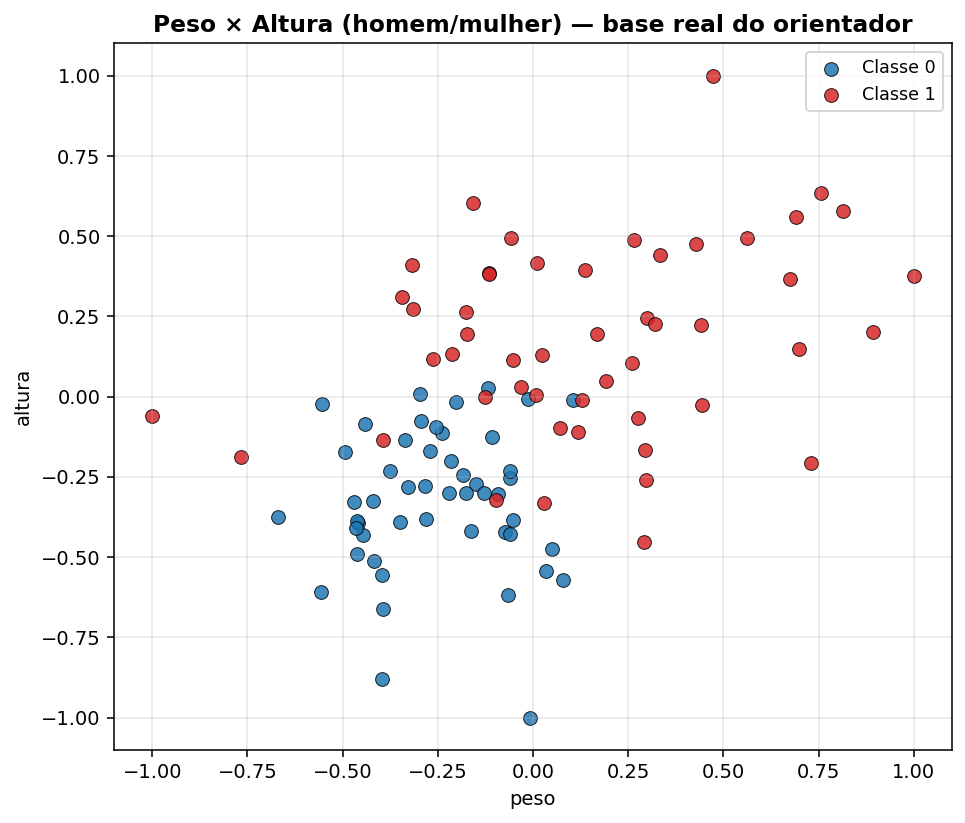
\includegraphics[width=\linewidth,height=0.7\textheight,keepaspectratio]{bloco3_01_peso_altura_overview.png}
  \end{columns}
\end{frame}

% ============ 58. Variantes prompt na base real ============
\begin{frame}{Bloco 3 --- Problema G (peso $\times$ altura) --- variantes de prompt}
  \footnotesize
  \textbf{Duas variantes:}
  \begin{itemize}
    \item \textbf{NEUTRA}: features = $(x_1, x_2)$. LLM sem prior sem\^antico.
    \item \textbf{SEM\^ANTICA}: features = $(\text{peso}, \text{altura})$. LLM ativa priors do treinamento.
  \end{itemize}
  \medskip
  Pergunta em ambas: \emph{homem ou mulher}.
\end{frame}

% ============ 59. Problema A R2/R3/R4 ============
\begin{frame}{Bloco 3 --- Problema G (peso $\times$ altura) --- aprendizado de $W$ com 2 / 3 / 4 features}
  \scriptsize
  \begin{center}
    
\includegraphics[width=0.85\linewidth,height=0.7\textheight,keepaspectratio]{bloco23_external_features_comparison.png}
  \end{center}
\end{frame}

% ============ 60. Acuracia REAL ============
\begin{frame}{Bloco 3 --- Problema G (peso $\times$ altura) --- acur\'acia vs r\'otulo REAL}
  \scriptsize
  \textbf{O que est\'a sendo feito:} para cada $n_{\text{feat}} \in \{2, 3, 4\}$ (R2, R3, R4), o LLM rotula os pontos em zero-shot com prompt \textbf{sem\^antico} (features ``peso'', ``altura''); estimamos $\hat W$ via otim.\ inversa. Reportam-se duas m\'etricas: (i) \textbf{fidelidade vs LLM} (NNLS reproduz r\'otulos do LLM) e (ii) \textbf{acur\'acia vs r\'otulo REAL} (homem/mulher --- ground truth humano). Exce\c{c}\~ao metodol\'ogica do Bloco 3 --- aqui medimos GT.
  \medskip
  M\'edia 3 seeds:
  \begin{center}
  \begin{tabular}{lccc}
    \toprule
    $n_{\text{feat}}$ & Fid.\ vs LLM (NNLS) & Acc.\ vs REAL (NNLS) & Observa\c{c}\~ao \\
    \midrule
    2 & 0{,}561 & 0{,}833 & --- \\
    3 & 0{,}624 & 0{,}838 & --- \\
    4 & 0{,}723 & 0{,}752 & fid sobe, acc real cai \\
    \bottomrule
  \end{tabular}
  \end{center}
  \medskip
  Em prompt \textbf{neutro} ($x_1, x_2$), acur\'acia REAL despenca para 30--40\% --- LLM perdido sem prior sem\^antico.
\end{frame}

% ============ 61. Paradoxo overfitting ============
\begin{frame}{Bloco 3 --- Paradoxo do overfitting --- prompt neutro $x_1/x_2$}
  \footnotesize
  Em peso $\times$ altura com prompt NEUTRO (3 seeds):
  \begin{itemize}
    \item Fidelidade Perceptron 2$\to$4 features: \textbf{sobe} ($\sim$60\% $\to$ 75\%).
    \item Acur\'acia vs real: \textbf{cai} (43\% $\to$ 40\%).
  \end{itemize}
  \medskip
  \textbf{Diagn\'ostico:} 4 pesos para 70 amostras de treino $\Rightarrow$ graus de liberdade suficientes para decorar ru\'ido das decis\~oes ERRADAS do LLM. Overfitting cl\'assico.
  \medskip
  \textbf{Mensagem:} subir $n_{\text{feat}}$ s\'o vale com n\~ao-linearidade real \emph{e} dados suficientes.
\end{frame}

% ============ 62. Peso x altura LLM como aprendiz ============
\begin{frame}{Bloco 3 --- Problema G (peso $\times$ altura) --- LLM como aprendiz}
  \scriptsize
  \textbf{O que est\'a sendo feito:} aplica a metodologia ``LLM como aprendiz'' (mesma do Bloco 2) ao problema real peso $\times$ altura. Para cada $n_{\text{shot}} \in \{0, 5, 10, 20, 40\}$, o LLM recebe exemplos rotulados com o \textbf{ground truth real} (homem/mulher) e classifica o conjunto de teste. Comparamos com tr\^es refer\^encias: \textbf{acc\_metric} (LLM vs $\hat W$ aprendida), \textbf{acc\_real} (LLM vs GT humano), e \textbf{baseline Perceptron} treinado nos mesmos exemplos. Prompt sem\^antico (``peso'', ``altura'').
  \medskip
  M\'edia 3 seeds:
  \begin{center}
  \begin{tabular}{lccc}
    \toprule
    $n_{\text{shot}}$ & acc\_metric & acc\_real & perceptron\_baseline\_real \\
    \midrule
    0  & 0{,}567 & 0{,}600 & --- \\
    5  & 0{,}833 & 0{,}778 & \textbf{0{,}917} \\
    10 & 0{,}944 & 0{,}867 & 0{,}778 \\
    20 & 0{,}944 & 0{,}844 & 0{,}822 \\
    40 & \textbf{0{,}989} & 0{,}889 & 0{,}878 \\
    \bottomrule
  \end{tabular}
  \end{center}
  \textbf{Achados:}
  \begin{itemize}
    \item LLM atinge 99\% acc\_metric com 40 exemplos.
    \item Em \textbf{5-shot}, Perceptron baseline supera LLM (91,7\% vs 77,8\%).
    \item Em $n_{\text{shot}} \geq 10$, LLM passa o Perceptron.
  \end{itemize}
\end{frame}

% ============ 63. Problema E curvas por variante ============
\begin{frame}{Bloco 3 --- Problema G (peso $\times$ altura) --- curvas LLM como aprendiz por variante}
  \scriptsize
  \begin{center}
    
\includegraphics[width=0.8\linewidth,height=0.75\textheight,keepaspectratio]{bloco23_external_learning_curve.png}
  \end{center}
\end{frame}

% ============ 64. LLM vs Perceptron peso x altura ============
\begin{frame}{Bloco 3 --- Problema G (peso $\times$ altura) --- LLM vs Perceptron baseline}
  \scriptsize
  \begin{center}
    
\includegraphics[width=0.85\linewidth,height=0.75\textheight,keepaspectratio]{bloco23_external_llm_vs_perceptron.png}
  \end{center}
\end{frame}

% ============ 65. Quando o LLM ganha ============
\begin{frame}{Bloco 3 --- Quando o LLM ganha?}
  \scriptsize
  \textbf{O que est\'a sendo feito:} compara\c{c}\~ao cruzada entre 3 cen\'arios em $n_{\text{shot}}=10$: (i) peso $\times$ altura com prompt sem\^antico, (ii) peso $\times$ altura com prompt neutro $(x_1, x_2)$, (iii) meia-lua. Mede \textbf{acur\'acia vs ground truth} do LLM contra o baseline Perceptron treinado nos mesmos exemplos. Isola \emph{quando} o LLM tem vantagem sobre um classificador cl\'assico.
  \medskip
  \begin{center}
  \begin{tabular}{lcc}
    \toprule
    Cen\'ario ($n_{\text{shot}}=10$) & LLM acc\_real & Perceptron baseline real \\
    \midrule
    peso/altura sem\^antico & \textbf{0{,}867} & 0{,}778 \\
    $x_1/x_2$ neutro        & 0{,}356 & 0{,}356 \\
    meia-lua                & 0{,}622 & \textbf{0{,}889} \\
    \bottomrule
  \end{tabular}
  \end{center}
  \medskip
  \textbf{Interpreta\c{c}\~ao:}
  \begin{itemize}
    \item LLM ganha com \textbf{priors sem\^anticos} (peso/altura).
    \item Em \textbf{features neutras}, ambos s\~ao igualmente ruins.
    \item Em \textbf{meia-lua}, Perceptron baseline (com augmenta\c{c}\~ao) ganha do LLM in-context.
    \item Vantagem do LLM vem dos \emph{priors do treinamento}, n\~ao do ICL per se.
  \end{itemize}
\end{frame}

% ============ 66. Visualizacao ponto-a-ponto 2 imagens ============
\begin{frame}{Bloco 3 --- Visualiza\c{c}\~ao ponto-a-ponto das rotula\c{c}\~oes do LLM}
  \scriptsize
  Atende adendo do e-mail 22:06.
  \begin{center}
    
\includegraphics[width=0.45\linewidth,keepaspectratio]{final_08_llm_labels_seed42_peso_altura_5.png}\hfill
    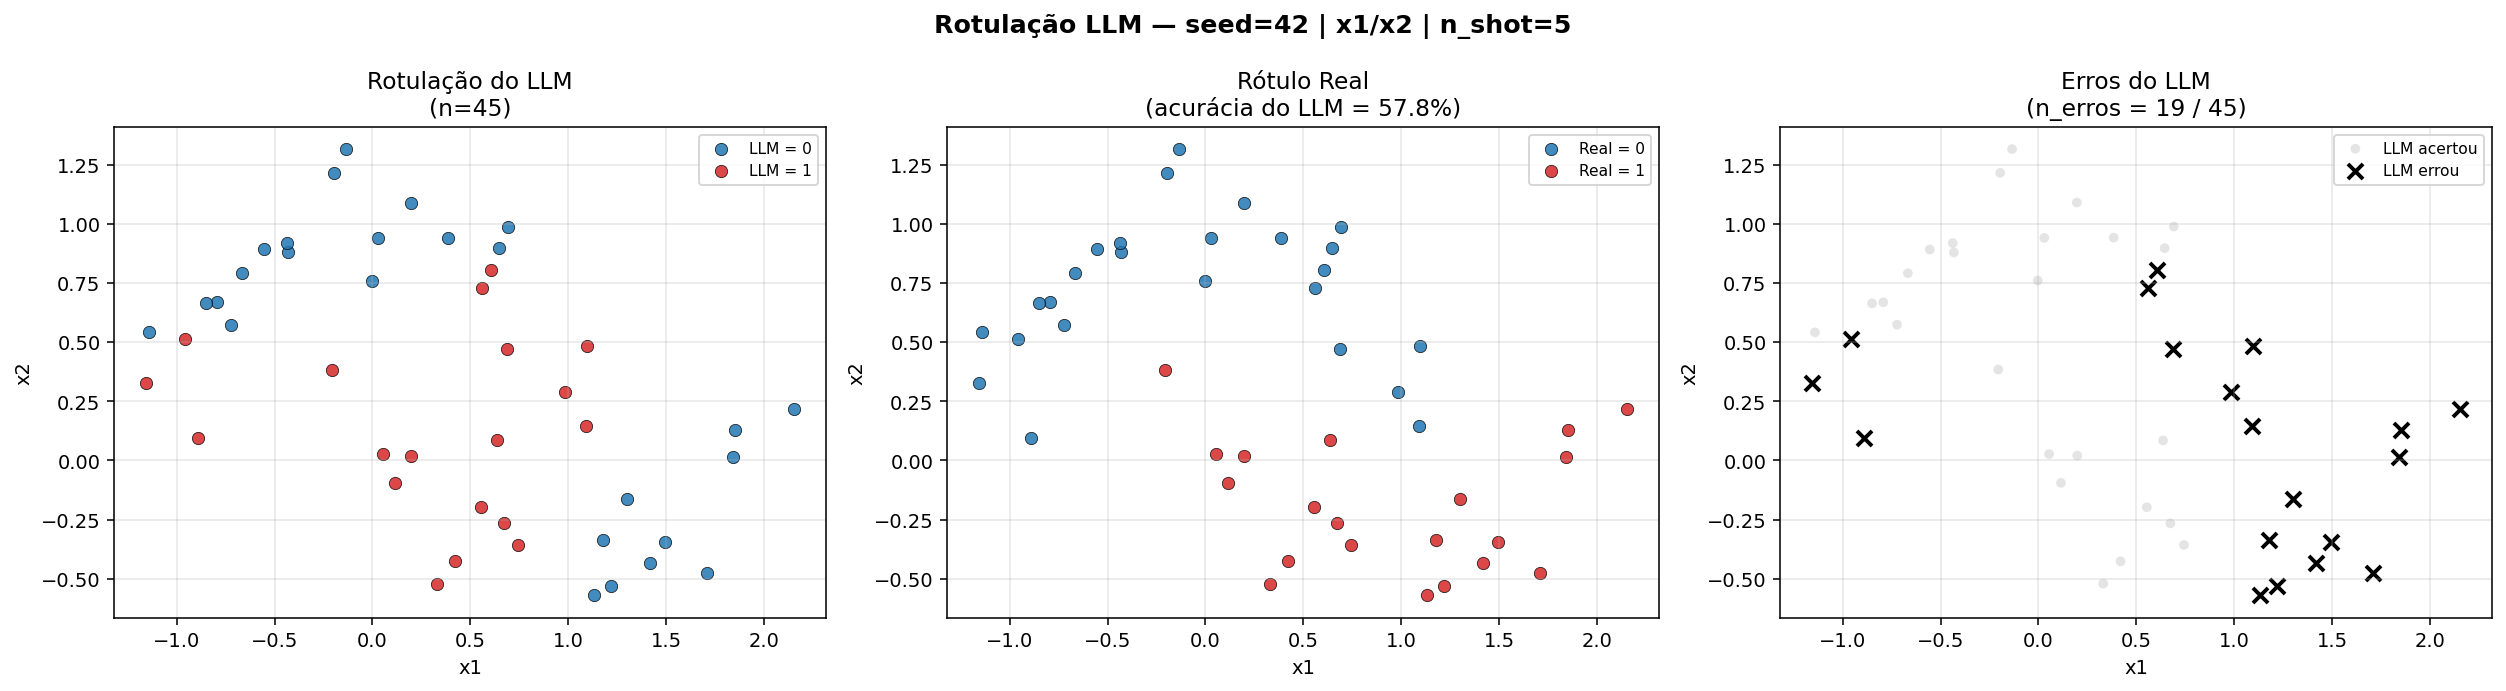
\includegraphics[width=0.45\linewidth,keepaspectratio]{final_08_llm_labels_seed42_x1_x2_5.png}
  \end{center}
  Esq.: prompt SEM\^ANTICO (peso/altura). Dir.: prompt NEUTRO ($x_1/x_2$). Mesmos pontos, classes muito diferentes.
\end{frame}

% ============ 67. Resumo Bloco 3 ============
\begin{frame}{Bloco 3 --- Resumo Bloco 3}
  \footnotesize
  \begin{itemize}
    \item \textbf{Priors sem\^anticos s\~ao reais}: peso/altura $\to$ 89\% acc\_real, $x_1/x_2$ $\to$ 36\%.
    \item \textbf{R4 (elipse)} recupera a forma te\'orica mas \emph{overfit-a} com 100 amostras.
    \item \textbf{LLM vs Perceptron} (5-shot peso/altura): Perceptron 92\% vs LLM 78\% --- com dados rotulados, m\'etrica cl\'assica \'e competitiva.
    \item \textbf{Conclus\~ao:} LLM ganha com priors + few-shot pequeno; perde para baselines com mais dados.
  \end{itemize}
\end{frame}

% ===== FECHAMENTO =====

% ============ 68. Sintese cruzada ============
\begin{frame}{S\'intese cruzada dos 3 blocos}
  \scriptsize
  Dados em \texttt{final\_cross\_linearity.csv} (mediana 3 seeds, NNLS):
  \begin{center}
  \begin{tabular}{lccc}
    \toprule
    Problema & R2$\to$R4 fid.\ & R2$\to$R4 acc\_real & Esperado \\
    \midrule
    A/B/C lineares       & +5 p.p.\ (ru\'ido)  & ---                  & sem ganho $\checkmark$ \\
    Meia-lua             & \textbf{+7,6 p.p.}  & $\sim$0 a +3 p.p.    & ganho $\checkmark$ \\
    Peso $\times$ altura & \textbf{+16 p.p.}   & \textcolor{red}{$-$25 p.p.\ (neutro)} & overfit $\times$ \\
    \bottomrule
  \end{tabular}
  \end{center}
  \medskip
  \textbf{Padr\~ao:} R3/R4 ajuda em n\~ao-linearidade real \emph{quando h\'a dados suficientes}.
\end{frame}

% ============ 69. Robustez entre seeds ============
\begin{frame}{Robustez entre seeds (3 seeds $\times$ 3 reps)}
  \scriptsize
  \begin{center}
  \begin{tabular}{lc}
    \toprule
    M\'etrica & M\'edia $\pm$ desvio \\
    \midrule
    Fidelidade Problema A        & $75{,}1\% \pm 8{,}4$ p.p. \\
    Consist\^encia Problema B    & $65{,}4\% \pm 7{,}0$ p.p. \\
    Consist\^encia Problema C    & $79{,}5\% \pm 7{,}1$ p.p. \\
    Kappa Problema B             & $0{,}19 \pm 0{,}13$ \\
    Kappa Problema C             & $0{,}49 \pm 0{,}23$ \\
    \bottomrule
  \end{tabular}
  \end{center}
  \medskip
  Desvio $< 8$ p.p.\ entre seeds --- \textbf{H5 sustentada}.
\end{frame}

% ============ 70. Testes principais ============
\begin{frame}{Testes estat\'isticos principais}
  \scriptsize
  \begin{center}
  \begin{tabular}{lcc}
    \toprule
    Compara\c{c}\~ao & $\Delta$ observado & Veredito \\
    \midrule
    Few-shot vs zero-shot (Problema E euclid) & $+0{,}38$ ($\sim$0.55$\to$0.93) & SIG \\
    Easy vs Hard ($n_{\text{shot}}=5$)    & $+0{,}258$ (0.78 vs 0.52)      & \textbf{SIG, H4 refutada} \\
    Easy vs Hard ($n_{\text{shot}}=40$)   & $-0{,}137$ (0.82 vs 0.96)      & SIG, REVERTIDO \\
    R2 vs R4 (meia-lua, fid)               & $+0{,}08$                       & SIG \\
    Cosseno $W_{\text{perc}}, W_{\text{nnls}}$ & 0{,}95+                  & robusto \\
    \bottomrule
  \end{tabular}
  \end{center}
  \medskip
  Diagn\'ostico de $\gamma$ no Perceptron (item b reuni\~ao 30/04, $\sim$520s): figura \texttt{final\_10\_gamma\_convergence.png} confirma converg\^encia monot\^onica.
\end{frame}

% ============ 71. Testes complementares ============
\begin{frame}{Testes estat\'isticos complementares}
  \footnotesize
  \begin{enumerate}
    \item \textbf{Point-biserial} (confian\c{c}a LLM $\times$ acerto): $r \approx 0{,}42$, $p<0{,}001$ --- LLM "sabe" quando tem certeza.
    \item \textbf{Mann-Whitney U} (margem em acertos vs erros): $p<0{,}001$ --- erros concentrados em pontos de baixa margem.
    \item \textbf{Kruskal-Wallis} (ordem de exemplos $\times$ acur\'acia): $H = 2{,}1$, $p \approx 0{,}55$ (n.s.) --- ordem n\~ao altera significativamente.
  \end{enumerate}
\end{frame}

% ============ 72. Sintese hipoteses ============
\begin{frame}{S\'intese das hip\'oteses (por bloco)}
  \footnotesize
  \begin{center}
  \begin{tabular}{llp{5cm}}
    \toprule
    Bloco & Hip\'otese & Veredito \\
    \midrule
    I  & H1 (consist\^encia)            & Sustentada parcial (Kappa C 0,49; Kappa B 0,19) \\
    I  & H2 (few-shot amplifica)        & \textbf{Sustentada} \\
    II & H3 (LLM como aprendiz)         & \textbf{Sustentada} (Problema E linear: +40 p.p.) \\
    II & H4 (exemplos dif\'iceis)        & \textcolor{red}{\textbf{REFUTADA}} em $n_{\text{shot}}$ pequeno; \emph{revertida} em $n_{\text{shot}}=40$ \\
    Trans. & H5 (estabilidade)         & \textbf{Sustentada} ($\sigma < 8$ p.p.) \\
    \bottomrule
  \end{tabular}
  \end{center}
\end{frame}

% ============ 73. Conclusoes ============
\begin{frame}{Conclus\~oes principais}
  \footnotesize
  \begin{enumerate}
    \item Existe um \textbf{crit\'erio decis\'orio est\'avel} no LLM (H1) --- ortogonal a corre\c{c}\~ao.
    \item \textbf{Few-shot amplifica} a concord\^ancia LLM--m\'etrica (H2).
    \item LLM \textbf{aprende crit\'erio de perito} via ICL (H3); baselines cl\'assicos competitivos com mais dados.
    \item \textbf{Easy} supera \textbf{hard} em poucos exemplos --- mas hard reverte em $n_{\text{shot}}=40$.
    \item \textbf{R3/R4} s\'o ajuda em problemas n\~ao-lineares E com dados suficientes (overfit em peso $\times$ altura com 100 amostras).
    \item Vantagem do LLM em peso $\times$ altura vem dos \textbf{priors sem\^anticos} do treinamento.
  \end{enumerate}
\end{frame}

% ============ 74. Limitacoes ============
\begin{frame}{Limita\c{c}\~oes}
  \footnotesize
  \begin{itemize}
    \item M\'etrica diagonal n\~ao captura intera\c{c}\~oes entre features.
    \item 2D apenas --- problemas reais s\~ao multidimensionais.
    \item Peso $\times$ altura tem s\'o 100 amostras (pouco para 4 features).
    \item 1 LLM testado (\texttt{gpt-4o-mini}).
    \item Sem controle de vers\~ao do LLM entre execu\c{c}\~oes (provider pode mudar).
  \end{itemize}
\end{frame}

% ============ 75. Agradecimentos ============
\begin{frame}{Agradecimentos}
  \footnotesize
  \begin{center}
    \Large \textbf{Obrigado!}
    \medskip

    \normalsize
    Orientador: Prof.\ Raul Fonseca Neto (UFJF)\\
    Programa de P\'os-Gradua\c{c}\~ao em Inform\'atica
    \medskip

    \large \textbf{Perguntas?}
  \end{center}
\end{frame}

% ===== APENDICE TECNICO =====

% ============ 76. A1 Perceptron ============
\begin{frame}{A1 --- Perceptron Estruturado (CILAMCE 2017)}
  \scriptsize
  Formula\c{c}\~ao primal (Eq.\ 28):
  \[ \max\ \gamma \quad \text{s.t.}\ d_W(x_i,c_k) - d_W(x_i,c_\ell) + \lambda\alpha_i \geq \gamma\|w\|,\ w \geq 0,\ \alpha \geq 0 \]
  Regra de corre\c{c}\~ao (Eq.\ 29):
  \begin{align*}
    w &\leftarrow w(1 - \eta\gamma/\|w\|) - \eta \cdot ((x_i-c_\ell)^2 - (x_i-c_k)^2) \\
    \alpha_i &\leftarrow \alpha_i + \eta
  \end{align*}
  Busca bin\'aria (Eq.\ 31): $\gamma^{(t+1)} \leftarrow \gamma^{(t)} + \Delta$. Hiperpar\^ametros do artigo: $\eta=0{,}001$, $C \in [0{,}1; 1{,}0]$.
\end{frame}

% ============ 77. A2 NNLS ============
\begin{frame}{A2 --- NNLS (Lawson \& Hanson 1974)}
  \scriptsize
  \[ \min_w \|Aw - b\|^2 \quad \text{s.t.}\ w \geq 0, \qquad A_{i,j} = (x_{ij} - c_{kj})^2 - (x_{ij} - c_{\ell j})^2,\ b_i = 1 \]
  M\'etodo de conjunto ativo via \texttt{scipy.optimize.nnls}. Tempo polinomial, determin\'istico, \'otimo global do problema convexo. Zero hiperpar\^ametros.
\end{frame}

% ============ 78. A3 Equivalencia ============
\begin{frame}{A3 --- Equival\^encia Perceptron $\leftrightarrow$ NNLS}
  \scriptsize
  \begin{center}
  \begin{tabular}{lcc}
    \toprule
    & Perceptron & NNLS \\
    \midrule
    M\'etodo  & Gradiente projetado & QP (Lawson-Hanson) \\
    Hiperpar.\ & $\eta, C, \Delta_\gamma$ & nenhum \\
    Determinismo & N\~ao & Sim \\
    \'Otimo global & N\~ao garantido & Garantido (convexo) \\
    \bottomrule
  \end{tabular}
  \end{center}
  Valida\c{c}\~ao emp\'irica nesta execu\c{c}\~ao: cosseno entre $W$'s $> 0{,}95$.
\end{frame}

% ============ 79. B1 Overfitting ============
\begin{frame}{B1 --- Overfitting com poucos dados}
  \footnotesize
  Caso emblem\'atico (peso $\times$ altura, $x_1/x_2$, 4 features, m\'edia 3 seeds):
  \begin{itemize}
    \item Fidelidade $\approx 75\%$ (m\'etrica decora as decis\~oes erradas do LLM).
    \item Acur\'acia vs real $\approx 40\%$ (LLM em si erra muito sem prior sem\^antico).
  \end{itemize}
  \textbf{Diagn\'ostico:} 4 pesos $\times$ 70 amostras de treino = decora ru\'ido.\\
  \textbf{Mitiga\c{c}\~oes:} regulariza\c{c}\~ao L1/L2, mais dados, CV $k$-fold, sele\c{c}\~ao autom\'atica.
\end{frame}

% ============ 80. C1 XAI ============
\begin{frame}{C1 --- XAI e otimiza\c{c}\~ao inversa}
  \footnotesize
  \begin{itemize}
    \item Ahuja \& Orlin (2001): formula\c{c}\~ao cl\'assica em PL.
    \item Schultz \& Joachims (2003): margem SVM-style.
    \item Coelho, Borges, Fonseca Neto (CILAMCE 2017): perceptron estruturado.
  \end{itemize}
  Diferencia\c{c}\~ao: aplica\c{c}\~ao a LLMs (interface texto), m\'etodo black-box, independente de arquitetura.
\end{frame}

% ============ 81. C2 ICL ============
\begin{frame}{C2 --- In-context learning e few-shot}
  \footnotesize
  \begin{itemize}
    \item Brown et al.\ (2020): GPT-3 e few-shot.
    \item Min et al.\ (2022): "no role of ground truth", "label space matters".
    \item Wei et al.\ (2022): emergent abilities.
    \item Lyu et al.\ (2023): prompts can\^onicos --- alinhado com refuta\c{c}\~ao H4 em few-shot pequeno.
  \end{itemize}
\end{frame}

% ============ 82. C3 Metric Learning ============
\begin{frame}{C3 --- Metric learning e Mahalanobis}
  \footnotesize
  \begin{itemize}
    \item Xing et al.\ (2002): original Mahalanobis metric learning.
    \item Davis et al.\ (2007): ITML.
    \item Schultz \& Joachims (2003): SVM-style margin.
    \item Diagonal: Liu et al.\ (2010), Kedem et al.\ (2012).
  \end{itemize}
\end{frame}

% ============ 83. D1 Pipeline + diagnostico gamma ============
\begin{frame}{D1 --- Reprodu\c{c}\~ao + diagn\'ostico $\gamma$}
  \scriptsize
  \texttt{python src/dissertacao\_mestrado.py}
  \medskip
  \begin{center}
    
\includegraphics[width=0.85\linewidth,height=0.55\textheight,keepaspectratio]{final_10_gamma_convergence.png}
  \end{center}
  Diagn\'ostico da busca bin\'aria em $\gamma$ (item b reuni\~ao 30/04 $\sim$520s): $\gamma_{\text{lo}}$ monot\^onico crescente confirma converg\^encia.
\end{frame}

% ============ 84. D2 Limitacoes reprodutibilidade ============
\begin{frame}{D2 --- Limita\c{c}\~oes de reprodutibilidade}
  \footnotesize
  \begin{itemize}
    \item LLM evolui silenciosamente entre execu\c{c}\~oes.
    \item Temperatura $0$ N\~AO garante determinismo (batching GPU).
    \item Usamos 3 seeds $\times$ 3 reps = 9 observa\c{c}\~oes/config.
    \item Estocasticidade residual t\'ipica $< 2\%$ entre reps da mesma seed.
  \end{itemize}
\end{frame}

\end{document}
